\documentclass[11pt]{article}
\usepackage[english]{babel}
\usepackage[utf8]{inputenc}
\usepackage{amsmath}
\usepackage{graphicx}
\usepackage{float}
\usepackage[letterpaper, margin=1in]{geometry}
\usepackage{tocloft}
\usepackage{setspace} \doublespacing
\usepackage{dcolumn}
\usepackage{comment}
\usepackage{longtable,booktabs,array}
\usepackage[authordate,backend=biber]{biblatex-chicago}
\addbibresource{2023-02-18.bib}
\usepackage[bottom]{footmisc}
\usepackage{caption}
\usepackage{hyperref}


\renewcommand{\cfttoctitlefont}{\hfill\Large\bfseries}
\renewcommand{\cftaftertoctitle}{\hfill\hfill}
\renewcommand{\cftloftitlefont}{\hfill\Large\bfseries}
\renewcommand{\cftafterloftitle}{\hfill}
\renewcommand{\cftlottitlefont}{\hfill\Large\bfseries}
\renewcommand{\cftafterlottitle}{\hfill}
% These 6 lines will center the titles of the table of contents, list of figures and list of tables

\begin{document}
\pagenumbering{roman}
\begin{titlepage}
\setcounter{page}{1}
\addcontentsline{toc}{section}{Abstract}
\begin{center}
\vspace{1cm}
\LARGE
\textbf{Land Use Restrictions and Segregation:\\ The Effect of Single-Family Zoning in Austin}



\Large
\vspace{.5cm}
%Subtitle: thesis presented for partial fulfillment...\\
\vspace{.5cm}
\textbf{Noah J. Case}\\
\vspace{.5cm}
\Large
\vspace{.5cm}
\large
\textbf{Abstract}
\end{center}


\begin{singlespace}
\noindent
I study the effect of zoning on segregation in Austin, Texas. I use municipal data on zoning for each address in Austin, and census data on demographics. I find that a one standard deviation increase in single-family zoning in a census block is associated with the population of that census block being 2.4 percentage points more White. To obtain a causal estimate, I restrict my sample to those census blocks directly adjacent to zoning boundaries. Next, I estimate the causal effect of a one standard deviation increase in single-family zoning to be that census blocks are 2.2 percentage points more White. Then, I adopt more sophisticated measures of segregation and test how those measures are related to zoning. Each measure I study leads to the same conclusion: single-family zoning contributes to segregation. Finally, I consider mechanisms for this effect, rejecting racial differences in income as the sole explanation for the zoning-segregation relationship.

\end{singlespace}
\vspace{0.4in}

\begin{figure}[H]
 \begin{center}
 
\includegraphics[width = .4\textwidth]{Vassar_Seal.pdf}
 \end{center}
 \end{figure}



\begin{center}	
Department of Economics\\
Vassar College\\
Poughkeepsie, New York\\
May 2, 2023\\
\end{center}
\end{titlepage}
\singlespacing
\setcounter{page}{2}
\tableofcontents
\pagebreak
\listoffigures
\listoftables
\pagebreak

    

\doublespacing

\begin{center}\section*{Acknowledgments}\end{center}
\addcontentsline{toc}{section}{Acknowledgements}

I wrote this thesis because I think that by enacting sound public policy governments can better the world. Knowing what those policies are is hard, but social sciences are up to the task. This thesis is dedicated to those whose lives might be improved by research like this.

I am in debt to the many people people who helped me write this thesis.

First, to my family---Mom, Dad, and Olivia---thank you for your love and support during the thesis process (and the twenty-one years that preceded it).

I gratefully acknowledge Professors Benjamin Ho and Dustin Frye, who were there at every step of this process with advice, guidance, and patience. They nurtured the germ of this thesis and saw it through to completion.

I cannot imagine a better major advisor than Professor Paul Johnson, who first suggested to me an Economics major in Spring 2020. He encourage me to challenge myself---and to go easy on myself when going easy was challenging.

I am especially grateful to Professor Lee Kennedy-Shaffer, who was my correlate advisor in Mathematics, and whose classes helped me think critically about how Statistics can serve humanity.


\pagebreak

\pagenumbering{arabic}
\doublespacing
\section{Introduction}
Expenditures on housing---typically either mortgage or rental payments---now make up more than one-third of annual consumer spending in the United States, with Blacks and Hispanics spending an even greater share of their incomes, despite being likelier to live in multi-family housing (Bureau of Labor Statistics 2022, Table B; Harvard JCHS 2017; Harvard JCHS 2011). One popular explanation for high housing costs is government regulations such as zoning (Quigley and Raphael 2004, page 205), which limits what kinds of housing can be built. Two stylized facts make the stakes of the zoning issue clear. First, Chakrabarti and Zhang (2005) find that a one unit increase in the city-level housing-price-to-income ratio reduces employment growth by 1.6 percentage points. Second, Hsieh and Moretti (2019) find that zoning reduced US GDP growth by 36 percent from 1964-2009.\footnote{Note that this figure is a very conservative estimate of the cost of zoning. First, they estimate the effects considering only three cities---New York, San Francisco, and San Jose. Second, their estimates assume that those three cities liberalize such that they are as restrictive as the median US city. But the median US city is zoned quite restrictively. The gains to complete liberalization would be much greater.} Though not the focus of this paper, zoning has macroeconomic consequences.

Turning my attention to race, I hypothesize that zoning causes segregation by diminishing the quantity of housing available, especially zoning that bans multi-family housing. Zoning is the set of laws and regulations that determine what type of housing can be built and in what quantities. It varies within \textit{and} between cities. I study variation in zoning within Austin, Texas. Segregation, for my purposes, is when there are significant differences in the racial composition of adjacent census blocks on either side of a zoning boundary. By limiting what sorts of housing can be built, and how many homes can be built on a single lot, zoning, functionally, is a leftward shift in the Housing Supply curve. Finally, although different zoning rules do different things, I expect that the zoning rules which cause the most segregation are bans on multi-family housing, in which Black and Hispanic people disproportionately live.

To test this hypothesis, I use zoning data from Austin and census block demographic data. I exploit plausibly-exogenous variation in zoning by restricting my dataset to include only census blocks directly adjacent to zoning blocks, so that the  blocks' zoning is as-if randomly assigned. I refer to this approach, which shares some characteristics with regression discontinuity design, as a geographic discontinuity design.

I find a statistically significant, socially meaningful effect of zoning on segregation. I also validate the methodology of other papers which have studied this issue, especially Resseger (2022), and contribute to a methodology to study the zoning question in other places as the requisite data becomes available. Finally, compared to Resseger, who studies the effect of zoning in Boston, I test whether the effects of zoning are different in a newer, larger, and more representative city. This means my estimates are more applicable to other cities than Resseger's. Boston is a unique city in the US---better educated, older, and with a distinct built environment---whereas Austin is more similar to typical American cities. I then explore some mechanisms by which zoning might cause segregation, and although I am not able to identify a specific mechanism, I reject the explanation than zoning causes segregation only because Whites are richer than non-Whites.

The causal estimate my paper obtains will be useful for cities seeking to change zoning in order to promote racial integration. Additionally, some of the most important changes to zoning will occur at the level of state legislatures, which are better able to overcome the coordination problems and perverse incentives which dominate local zoning decisions (Kazis 2022). Additionally, states---or even the Federal Government---could compel municipalities to release the zoning data that makes research like this possible. This would enable future scholars to study to impact of zoning on a broader scale.

\section{Literature Review}

The existing literature studying the economics of zoning suffers from two problems. First, its methods are rudimentary, and mostly do not address causality. Second, this literature has largely ignored racial questions. Additionally, though there are well-known racial disparities in access to housing, more work is needed to connect these disparities to zoning. I summarize the literature with these problems in mind.

\subsection{Coase Theorem}

The earliest work on the economics of zoning and land use restriction is purely theoretical. Much of it is motivated by Ronald Coase’s (1960) seminal paper on externalities. Coase demonstrates that incomplete assignment of property rights leads to market failures, but that complete assignment of property rights can remedy these failures.\footnote{Under the assumptions of costless bargaining and perfect information.} A memorable example from his paper is a confectioner whose workshop impedes a physician’s operation of his practice (page 9). This is the sort of problem zoning attempts to solve by separating incompatible land uses. However, Demetz (1964, page 23) warns of  rigid zoning’s costs, even when jurisdictions implement zoning to mediate the real harms from negative externalities. Still, Demetz does not empirically measure zoning’s costs.

Work on the economics of zoning, though, began in earnest in the 1970s. William Fischel (1978) formalizes the Coasean analysis of zoning. He criticizes zoning as an incomplete assignment of property rights, since (under typical zoning) no bargaining can occur between landowners and local governments, who hold the implicit property right to build (page 66); residents struggle to collectively actuate that property right. This theory guides research and offers one mechanism for the potential harms of zoning. However, at the same time, other researchers find that zoning has no effect on land prices, \textit{contra} Fischel (Maser et al 1977, page 128). Unfortunately, methodological problems with this early empirical work complicate a straightforward interpretation of their findings. Maser et al use appraisals to estimate land values. However, appraisals suffer from bias, and that bias may be endogenous to zoning.\footnote{They also only use one-sixth of the available data, which diminishes the power and credibility of their tests. I suspect this is due to the limited computing power at their disposal at the time the study was published.}

The earliest thorough examination of land use economics is William Fischel’s (1985) monograph, \textit{The Economics of Zoning Laws}. He criticizes the several studies which find home values are unaffected by proximity to non-conforming uses because those studies (Grether and Miezkowski 1980; Mark and Goldberg 1981) fail to control for the amenity provided by the nonconforming use. For instance, a factory may provide employment, but may also make adjacent land less desirable. Authors who fail to control for the employment amenity will produce a biased estimate of the effect of the factory on home prices (Fischel 1985, page 234-237). Other studies Fischel reviews measure the effect of zoning on home prices. He shows that a preponderance of studies find that zoning increases housing prices. Finally, Fischel provides a convincing theoretical explanation of why artificially high housing prices are bad, grounded in the models of urban economics. High prices drive people further from metropolitan cores which increases commute costs, lead people to buy smaller homes than they would otherwise be able to, and threaten to override the agglomerative benefits associated with cities (Fischel 1985, page 248). Fischel makes clear the need for more nuanced evaluations of zoning, as he finds fault with studies that find no effect from zoning and studies finding no effect from non-conforming uses. We need new empirical tools to gather evidence that does not have these problems.

\subsection{Early Empirical Work}

Better research methods enable more credible estimates of zoning’s effects. One breakthrough was Case and Shiller’s (1987) home price index, which for the first time avoids bias due to compositional effects.\footnote{The problem with estimating a change in average home values by simply averaging the sale prices of houses sold in two periods is that, if, for instance, preferences change so that in the first period, mostly small homes are sold, and in the second, mostly mansions are sold, we will estimate a spurious increase in the average home value. Case and Shiller base their estimates on only those homes which are sold twice (once in each period), avoiding this source of bias.} This quickly became the gold standard for home price data and is used in research on housing policy to the present day as an objective measure of home prices.\footnote{This index was purchased by S\&P Global Ratings, which now calculates it nationally.} However, this work is purely descriptive, and does not analyze any potential causes of changes in home prices. Fortunately, other scholars used this new methodology to estimate the effects of zoning. A study of jurisdictions in Montgomery County, Maryland, constructs an index of housing prices and land use restrictiveness. The study finds a statistically significant association between restrictive zoning and high home prices (Pollakowski and Wachter 1990, page 320). This study is the most credible estimate yet of the association between zoning and home prices, but it is not a causal estimate, because it fails to account for endogeneity. Although the authors control for income, they do not control for wealth or other measures of socioeconomic status which might cause confounding, as I demonstrate below.

Failure to account for endogeneity is a common problem in the economics of zoning literature. Consider a simple model regressing home prices, \textit{HP}, on a measure of zoning restrictiveness \textit{Z}. A positive fitted coefficient on \textit{Z} may reflect that zoning \textit{causes} higher home prices.\footnote{After all, there is ample theoretical reason to conclude that restrictive zoning causes higher home prices.} But it may also reflect that in affluent communities, wealthy home buyers bid up home prices, and those same wealthy voters have a preference for restrictive zoning. Research that does not account for this endogeneity cannot produce a credible causal estimate of zoning’s effects; researchers need more sophisticated models and methods, a point Quigley and Rosenthal (2005, page 84) emphasize. Mindful of this, I address the endogeneity problem with my narrow corridor approach, which offers credible estimates of the effect of zoning on segregation.

\subsection{Measuring Restrictiveness}

So far in this literature review, I discuss measurements of zoning’s costs. But another challenge is measuring zoning itself. Although there is interesting work occurring now on the creation of a so-called National Zoning Atlas (Bronin 2022), the best national information about zoning restrictiveness comes from the Wharton Residential Land Use Restrictive Index (WRLURI). The authors conduct a comprehensive survey of zoning and land use practices in 2600 US jurisdictions and create economists’ most valuable dataset on restrictiveness (Gyourko, Saiz, and Summers 2008). Then, in 2019, Gyourko et al recalculated the index based on 2019 data, finding that regulations had become more stringent in the intervening period (Gyourko, Hartley, and Krimmel 2019). Although this work is purely descriptive, the availability of the measure at two times allows for analysis of changes in restrictiveness over the past two decades.

Integrating the Wharton data, Gyourko and Krimmel (2021) calculate “zoning taxes” for the 24 largest Core Based Statistical Areas (CBSAs). They find that zoning taxes---the artificial increase in the price of developable vacant land---are highest in the most regulated cities, and highest nearest to city centers. However, they do not study race, so it is unknown whether different racial groups face different zoning taxes. In this study, I use by-address data to study the impact of zoning directly. This granularity allows me to avoid the potential issues involved in constructing aggregates measures of zoning restrictiveness.

\subsection{Addressing Race}

Over the past decade, scholars have studied the role of race more explicitly, using modern empirical techniques. Resseger (2022) finds that restrictive zoning in the Boston metropolitan area is partially responsible for racial segregation. He uses publicly available Massachusetts zoning data and census block demographic information, and studies racial demographics within a narrow corridor on either side of a zone boundary, which controls for confounding. He finds that permitting multi-family buildings by right leads to a 3.38 percentage point increase in the Black population and a 5.77 percentage point increase in the Hispanic population (page 33). As is well known, Boston has a unique history of segregation and racial strife.\footnote{For more information on this subject, see Bluestone and Stevenson (2000, Chapters 6-7).} I study these issues in a different setting, assessing whether Resseger’s findings hold elsewhere.


However, new research has also made clear that endogeneity concerns cannot be dismissed. Shertzer, Twinam, and Walsh (2015) hypothesize that in Chicago, Black neighborhoods were likelier to be zoned for industrial uses because of discrimination by city planners, especially in areas populated by Blacks from the South.\footnote{Chicago was zoned in 1923, during the Great Migration.} They use archival data from Chicago’s zoning commission and census demographic data to explore this question, finding that “a standard deviation increase in Black (first-generation immigrant) share increases the likelihood that a neighborhood received any manufacturing zoning by 5.4 (6.8) percentage points relative to native [W]hites” (page 237). This is compelling evidence that zoning is not exogenous of race, and given that contemporary neighborhood demographics are not exogenous of historical demographics, it is a reason to be cautious about causal inference in this area. I account for this endogeneity with the geographic discontinuity approach.

\subsection{Measuring Segregation}
The primary concern of my paper is measuring the causal role of zoning in segregating communities. However, this question elides the difficult task of measuring segregation. I begin with a simple measure---the share of a given census block's population who are White. Detecting a causal effect of zoning on the White share is an important task. However, this is a coarse measure of segregation. There is a rich literature---in economics, sociology, and biology---attempting to define and empirically measure segregation. I describe below several measures of segregation, each of which I calculate in Austin, and consider as an outcome in my analysis. 

The Herfindal-Hirschman\footnote{See Hirschman (1964) for an explanation of this index's name.} Index (HHI) was developed as a way to measure market concentration in various industries, by summing the squares of each firm's market share (Herfindahl 1950, page 19). We can apply a similar measure to race by summing the squares of each racial group's share of the population as below, 

\begin{equation}
    \text{HHI}=\sum_{i=1}^n \left(\frac{\text{Population}_i}{\text{Population}}\right)^2
\end{equation}

\noindent where $\text{Population}_i$ is the population of the \textit{i}th racial group in a given area, and Population is the total population in that area.\footnote{Biologists use the same formula to measure species diversity, though they call it the Simpson (1949) Index} This measure does not allow for easy comparison across geographies. Furthermore, it does not measure the way individuals of different races are distributed within a geographic area---it only counts their number. Advantageously, the HHI is simple to calculate and is calculable for any number of racial categories, and is familiar to readers from many fields of economics.

More sophisticated measures of segregation, such as the index of dissimilarity (Jahn, Schmid, and Schrag 1947) and the index of exposure permit distributional considerations, but allow only for comparisons between two groups, (e.g., Blacks and Whites, above or below the poverty line, etc.). For my purposes, the relevant comparison is between Whites and non-Whites. The dissimilarity index $D$, shown below, is a measure of the mean absolute deviation of each parcel's demographics from the demographics of the whole geographic unit (White 1964, page 202). For each parcel $i$, $\text{White}_i$ is the White population, and $\text{non-White}_i$ is the non-White population.

\begin{equation}
    D=\frac{1}{2}\sum_{i=1}^N\left|\frac{\text{White}_i}{\text{White}_{total}}-\frac{\text{non-White}_i}{\text{non-White}_{total}}\right|
\end{equation}

\noindent The other dichotomous measure of segregation I consider is the index of exposure (Blau 1977). Part of a family of indices which measure the probability of interactions between different groups, the index I describe in Equation 3 calculates the probability $E$ a non-White person will interact with a White person.

\begin{equation}
    E=\sum_{i=1}^n\left(\frac{\text{non-White}_i}{\text{non-White}_{total}}\right)\left(\frac{\text{White}_i}{\text{Population}_{i}}\right)
\end{equation}

\noindent For a brief proof that $E$ is this probability, see Appendix A.\footnote{Note this measure is asymmetric---in a mostly-White neighborhood, most Whites' interactions are with other Whites, and most Blacks' interactions are with Whites. The probability a White person interacts with a Black person is low, yet the probability a Black person interacts with a White person is high.} Although each of these measures improves upon the HHI, dichotomous models are less useful in Austin, where there are many Hispanics and Asians.

The index of segregation most appropriate in the case of polytomous segregation is the entropy index. This calculation can measure geographic segregation amongst any arbitrary number of groups, although it is less interpretable than those indices discussed above (White 1986, page 200). A parcel with $n$ racial groups has an entropy index $H$ given by

\begin{equation}
    H=-\sum_{i=1}^n\text{share}_i \log(\text{share}_i)
\end{equation}

\noindent where $\text{share}_i$ is the share of the population belonging to the \textit{i}th racial group. By convention, $0\log(0)$ is defined to be $0$. Finally, we have an index that combines the desirable properties of the HHI and the dissimilarity and exposure indices.\footnote{Inspired by renewed interest in segregation and dissatisfaction with traditional measures, Echenique and Fryer (2007) propose a new index of segregation which measures segregation at the level of an individual. My data does not allow me to calculate this measure, so I do not.} The formulae for $E$ and $D$ mean that those indices can be computed for only the \textit{second-most} granular geography one has data on. I calculate these for census tracts, rather than census blocks, and accordingly do not use them as regression outcomes. I do consider them, though, as indicators of segregation.


\section{Empirical Strategy}
I devise an empirical strategy to estimate the causal effect of single-family versus multi-family zoning on racial demographics. I use data from Austin, Texas to produce the estimate.

\subsection{Data}
I employ data from three sources. The first is Austin’s by-address zoning data (City of Austin 2020). This data gives, for each address in the city (\textit{ca.} 258,000), the type of zoning. With these addresses, I use the Census Bureau Batch Geocoding Service (Census Bureau n.d.) to obtain more specific information about each address, including its zip code, census tract, census block group, and census block. I merge the geocoding results file back to the original zoning information file as made available by Austin’s municipal government. So, for each address, I know the zone type and the relevant geographies. For this study, those geographies are the census tract and census block. In Figure \ref{fig:address_histogram}, I show a histogram of single-family zoning in all Austin census blocks. Although there are obvious concentrations of all single- and all multi-family zoning, the graph indicates that there is sufficient variation to use single-family zoning as a regressor in my models.

\begin{figure}
    \centering
    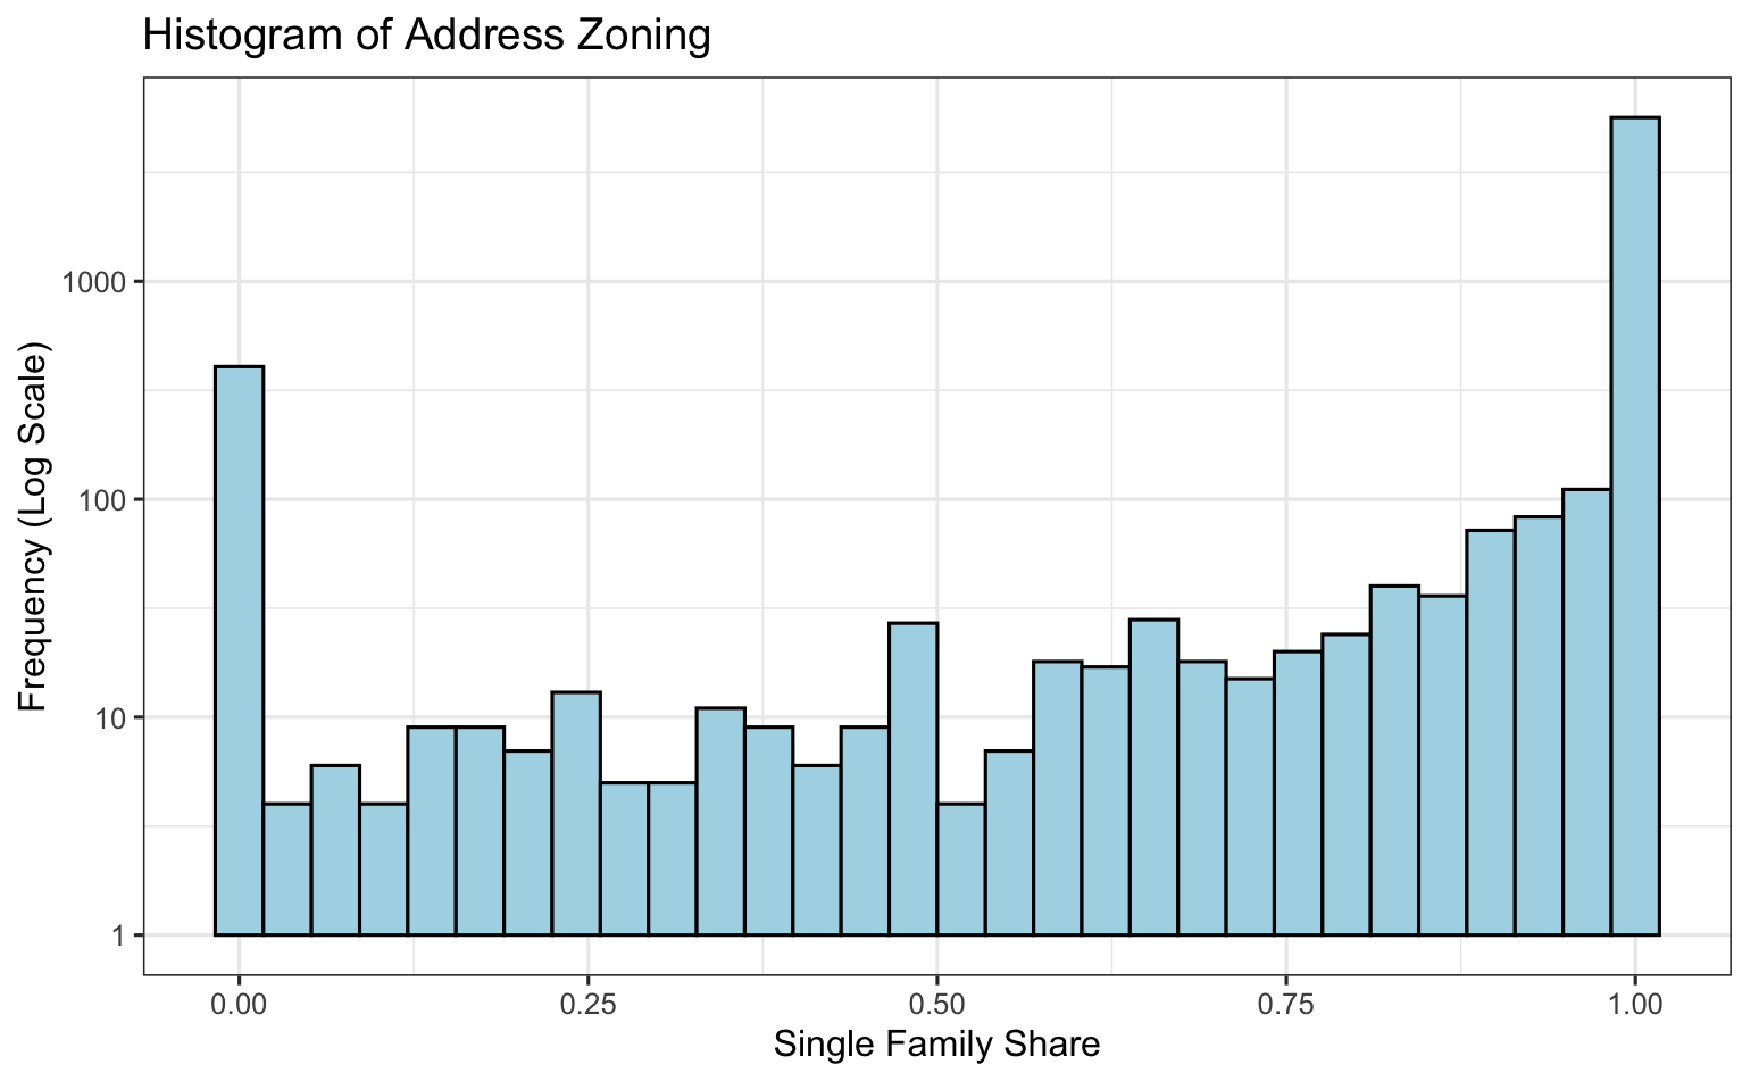
\includegraphics[width=\textwidth]{By_Block_Histogram.pdf}
    \caption{Histogram of Austin Census Blocks by Share of Single-Family Addresses}
    \label{fig:address_histogram}
\end{figure}

The next data I use is the Census Bureau’s (2022a) racial demographic information for 2020. The Census Bureau has information on the population and racial composition of each census block. Additionally, I obtain data from the American Community Survey (2020) on income at the census tract level, which will stand in for census block income, because to the best of my knowledge, income information is not available at the census block level.\footnote{For a detailed look at the Census Bureau’s geographies, see Rossiter (2014). For my purposes, it will suffice to know that census blocks are the smallest geography for which data is collected, and that census tracts are the union of census blocks. In Austin, there are \textit{ca.} 17,000 census blocks and \textit{ca.} 300 census tracts.} I use this data to control for the well-known association between neighborhood income and neighborhood racial composition.

Finally, I employ a map and a corresponding shapefile for use in \textit{QGIS}. The map shows each census block in Austin (Census Bureau 2020b). I merge a file containing demographic information and zoning information for each census block to the shapefile, which encodes geographic information about each census block's location. I generate a map, shown as Figure \ref{fig:Austin_Zoning_Map}, of Austin census blocks, colored by the share of addresses in each block zoned for single-family homes with QGIS.\footnote{Because some census blocks have no residential addresses, those blocks are excluded from the map. That accounts for `holes' scattered throughout the city. Also, the Colorado River flows through Austin from West to East, accounting for the apparently missing stripe through the middle part of the city.}

The map illustrates several facts about Austin's land use regime. First, the vast majority of land is colored red, indicating it is zoned for all or nearly all single-family homes. Second, there are very few blocks colored beige---these are blocks where both single- and multi-family homes are common. In general, Austin's zoning code separates these land uses. Third, there are many areas where no one lives, either because those areas are devoted to infrastructure such as highways or railroads, or because those areas are entirely commercial and industrial. This is similar to the patterns of land use in other American cities. I include other maps of Austin based on the Exposure, Dissimilarity, Entropy, and Herfindahl-Hirschman Index at the census tract and block level in Appendix B

%Fix formatting: Crop and move legend
\begin{figure}
    \centering
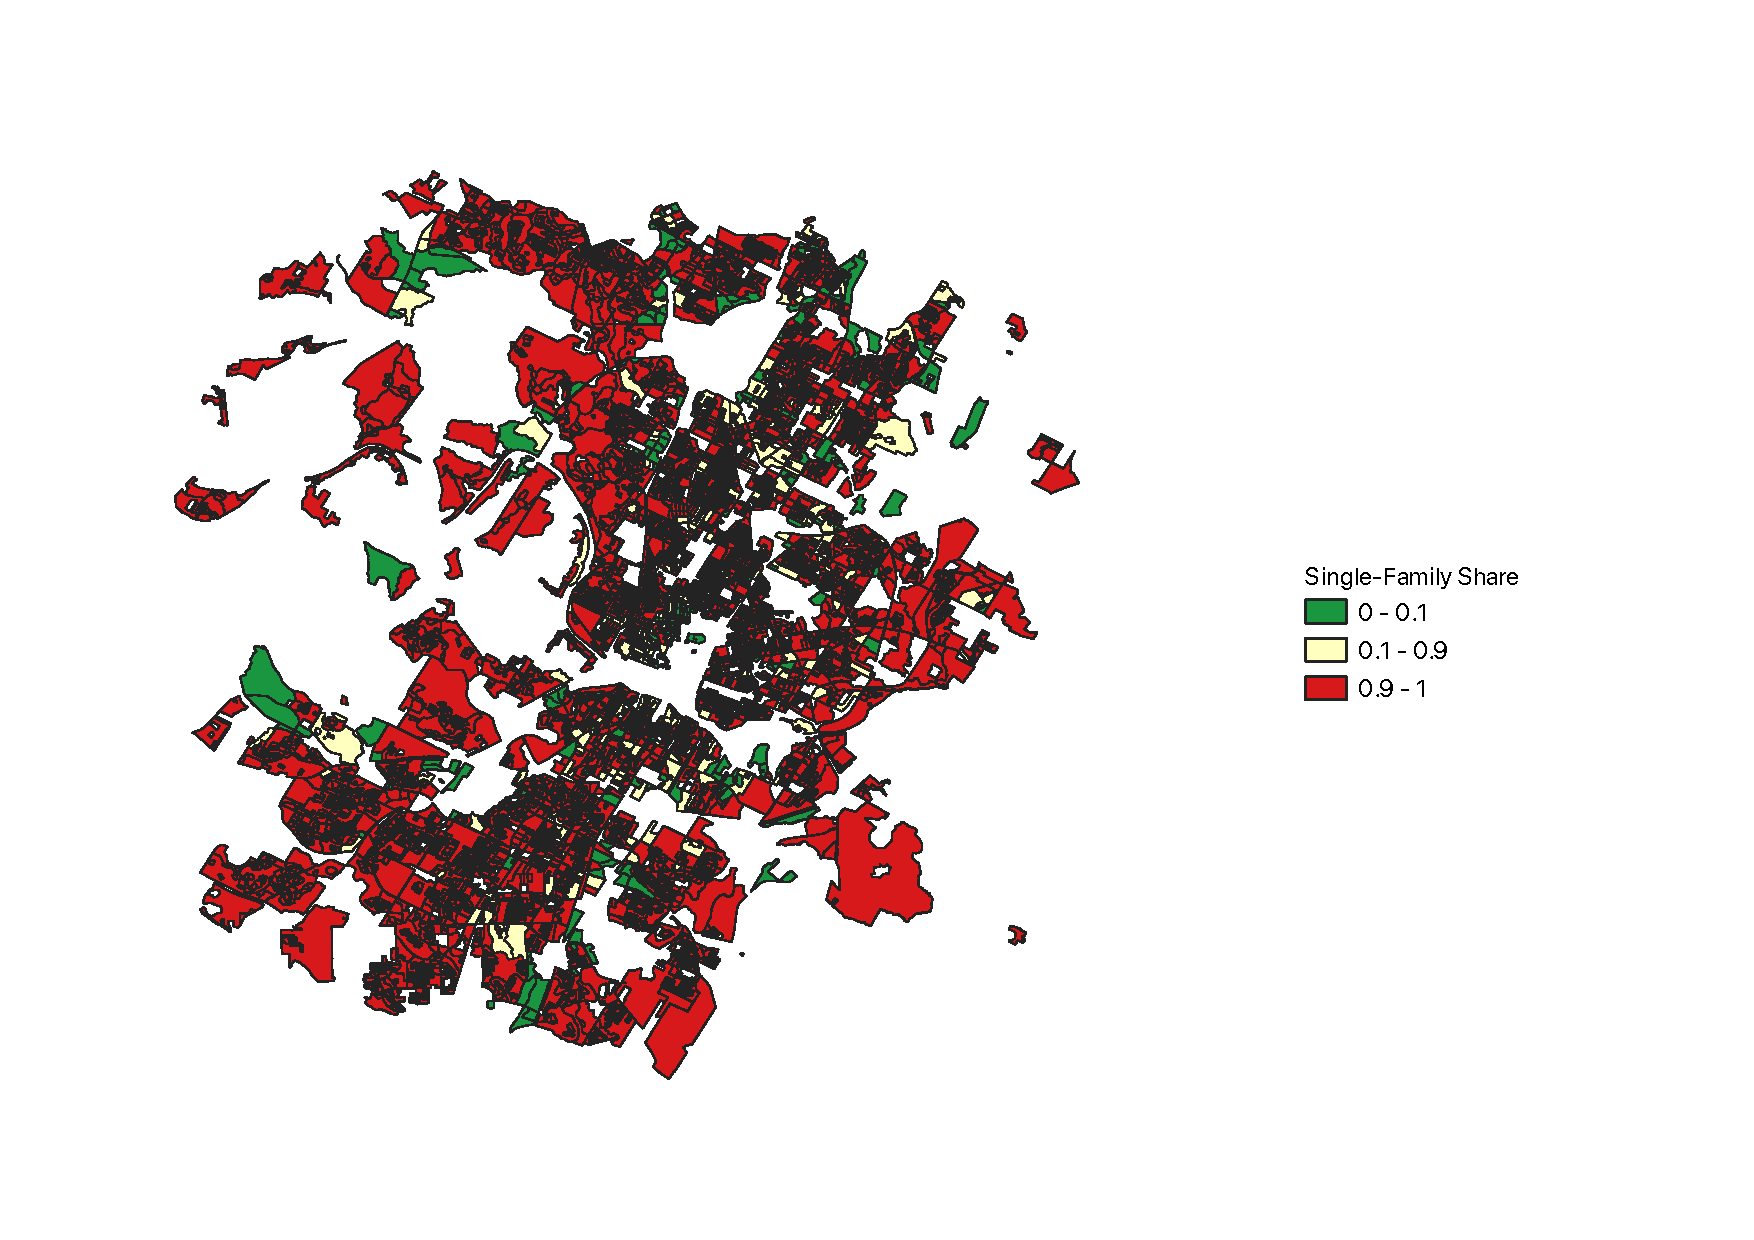
\includegraphics[width=\textwidth]{fig1_redone_output.pdf}
    \caption{Map of Austin Census Blocks Colored by Zoning}
    \label{fig:Austin_Zoning_Map}
\end{figure}

I choose census blocks for inclusion in the boundary dataset by identifying when adjacent census blocks are zoned for all single- and all multi-family homes. This step is necessary because, following Resseger (2022), my identification strategy is to study only those blocks directly adjacent to zoning boundaries in a geographic discontinuity design. I select blocks which border differently-zoned blocks. However, I exclude those blocks where there is a natural border or separation other than zoning. These include commercial areas, highways, the Colorado River, etc. For more information on the process of selecting blocks for inclusion in the boundary dataset, see Appendix C, where I include several figures and explain my criteria in greater depth. This approach has several advantages. In particular, because the boundary dataset is a subset of the full dataset (as opposed to being from a different source), its formatting is identical. All the analyses I perform on the boundary dataset I can perform on the dataset covering the whole zoned area, and vice versa.

\subsection{Summary Statistics}

\subsubsection{Entire Zoned Area}


\begin{table}[!htbp] \centering 
  \caption{Summary Statistics, All Census Blocks (N=6250)}
  \label{tab:Austin_summary_stats} 
\begin{tabular}{@{\extracolsep{5pt}}lccccc} 
\hline
\hline
\\[-1.8ex] 
Variables & Mean & Median & SD & Min & Max\\
\\[-1.8ex] \hline\\[-1.8ex] 
Population & 102.623 & 57.000 & 177.613 & 1 & 4299.0 \\
Share Non-Hispanic-White & 0.504 & 0.531 & 0.262 & 0 & 1.0 \\
Share Black & 0.062 & 0.021 & 0.096 & 0 & 1.0 \\
Share Asian & 0.064 & 0.027 & 0.099 & 0 & 1.0 \\
Share AIAN & 0.013 & 0.000 & 0.035 & 0 & 1.0 \\
Share NHPI & 0.001 & 0.000 & 0.012 & 0 & 0.5 \\
Share Other & 0.099 & 0.049 & 0.131 & 0 & 1.0 \\
Share Multiracial & 0.187 & 0.159 & 0.138 & 0 & 1.0 \\
Share Hispanic & 0.303 & 0.240 & 0.236 & 0 & 1.0 \\
SF-Zoned Addresses & 0.914 & 1& 0.257 & 0 & 1\\
Median Household Income & 95,227 & 83,365 & 39,323 & 6322 & 228,929 \\
HHI &5029 & 4773 & 1587 & 101 & 10,000  \\
Entropy Index & 0.8049 &	0.8217 & 0.2708 & 0 & 1.528 \\
\hline
\hline
\multicolumn{6}{l}{\textit{Note:} For Austin as a whole, $HHI=3544$ and $H=1.148$}\\ 
\end{tabular}
\end{table}


I begin by calculating and presenting summary statistics for Austin census blocks’ racial composition, population, median income, and segregation measures shown in Table \ref{tab:Austin_summary_stats}. These summary statistics  offer a sense of typical census block populations and racial shares. Of particular note are the two groupings for indigenous people---AIAN\footnote{American Indian/Alaska Native and Native Hawaiian/Pacific Islander respectively.} and NHPI---each of which has a median population of zero, implying that in more than half of census blocks there are no indigenous people. These summary statistics demonstrate that there is sufficient variation in the White Share to use this as the outcome variable in my regressions.

Next, I calculate summary statistics for the by-address data on Austin zoning, shown in Table \ref{tab:zone_freqs}. Notice that the zoning categories I display account for only about 75 percent of addresses in Austin. These are the major single- and multi-family categories in the Austin zoning code, so I focus on them. There are several categories I exclude: I exclude “Planned-Unit Developments” because those can be single- or multi-family, various commercial addresses, and other special categories which have only a few addresses, for example, airport areas and liquor stores. The single-family categories account for almost seventy percent of total addresses, and the multi-family categories account for about three percent of addresses. This is typical of American land use patterns, where most land is allocated toward single-family housing.

\begin{table}[!htbp] \centering 
  \caption{Summary Statistics for Austin Addresses} 
  \\[1.8ex]  \label{tab:zone_freqs} 
\begin{tabular}{@{\extracolsep{5pt}}llc} 
\hline\hline\\[-1.8ex] 
Zone & Number & Frequency \\
\\[-1.8ex] 
\hline
\\[-1.8ex] 
All & 258,136 & 1.000 \\
Single-Family Residence & 76,739 & 0.297 \\
Single-Family Standard Lot & 74,782 & 0.290 \\
Single-Family Small Lot & 16,309 & 0.063 \\
Single-Family Large Lot & 7755 & 0.030 \\
Multi-Family Limited Density & 3174 & 0.012 \\
Multi-Family Moderate Density & 2844 & 0.011 \\
Multi-Family Moderate High Density & 1558 & 0.006 \\
Multi-Family High Density & 217 & 0.001 \\
\hline\hline
\end{tabular}
\end{table}
\noindent 

\subsubsection{Boundary Subset}

I also calculate summary statistics for the census blocks included in the boundary subset of my data in Table \ref{tab:causal_summary_stats}. The blocks in the boundary subset are broadly similar to those in the whole city in terms of race, although they are somewhat poorer. They are also much more populous, which is probably related to the fact that they have more multi-family zoning (by construction of the dataset) than the blocks making up the whole zoned area. Finally, in Table \ref{tab:balance_table} I present a balance table for the blocks in the causal table, comparing the blocks zoned for single- and multi-family housing. I calculate and report $p$-values with Welch's unequal variance $t$-test.

\begin{table}
\caption{Summary Statistics, Boundary Subset (N=332)}
\\[1.8ex]
\label{tab:causal_summary_stats}
\centering
\begin{tabular}[!htbp]{@{\extracolsep{5pt}}lccccc} 
\hline
\hline
\\[-1.8ex] 
Variables & Mean & Median & SD & Min & Max\\
\hline\\[-1.8ex] 
Population & 228.401 & 94.000 & 324.142 & 3.000 & 2152.000 \\

Share Non-Hispanic-White & 0.505 & 0.521 & 0.236 & 0.000 & 0.949 \\

Share Black & 0.085 & 0.046 & 0.120 & 0.000 & 0.767 \\

Share Asian & 0.067 & 0.039 & 0.095 & 0.000 & 0.782 \\

Share AIAN & 0.012 & 0.000 & 0.029 & 0.000 & 0.263 \\

Share NHPI & 0.001 & 0.000 & 0.009 & 0.000 & 0.125 \\

Share Other & 0.100 & 0.069 & 0.110 & 0.000 & 0.562 \\

Share Multiracial & 0.159 & 0.135 & 0.107 & 0.000 & 0.875 \\

Share Hispanic & 0.288 & 0.235 & 0.189 & 0.000 & 0.895 \\

Median Household Income & 71,150 & 71,467 & 25,912 & 6322 & 228,929\\

SF-Zoned Addresses & 0.597 & 0.972 & 0.483 & 0.000 & 1.000 \\

HHI & 4655 & 4399 & 1447 & 1562 & 9007 \\
Entropy Index & 0.893 & 0.918 & 0.247 & 0.144 & 1.451 \\
\hline
\hline
\end{tabular}
\end{table}

\begin{table}[!htbp] \centering 
  \caption{Comparison Between Single- and Multi-Family Blocks, Boundary Subset} 
  \label{tab:balance_table} 
\begin{tabular}{@{\extracolsep{5pt}} lccccl} 
\\[-1.8ex]\hline 
\hline \\[-1.8ex] 


&\multicolumn{2}{c}{\textit{S-F Blocks }(N=200)}&\multicolumn{2}{c}{\textit{M-F Blocks }(N=132)}\\
 \cline{2-3} \cline{4-5}
 \\[-1.8ex] 
 Variables & Mean & SD & Mean & SD & \textit{p}-value\\ 

\hline \\[-1.8ex] 
Population & $159.825$ & $236.008$ & $332.303$ & $403.494$ &0.000\\ 
Share Non-Hispanic-White & $0.538$ & $0.236$ & $0.456$ & $0.228$ & 0.00187\\ 
Share Black & $0.072$ & $0.115$ & $0.106$ & $0.126$ &0.129\\ 
Share Asian & $0.057$ & $0.086$ & $0.082$ & $0.104$ &0.0204\\ 
Share AIAN & $0.014$ & $0.034$ & $0.009$ & $0.018$ & 0.0700\\ 
Share NHPI & $0.001$ & $0.008$ & $0.001$ & $0.011$ & 0.978\\ 
Share Other & $0.091$ & $0.106$ & $0.112$ & $0.114$ & 0.0923\\ 
Share Multiracial & $0.162$ & $0.105$ & $0.155$ & $0.111$ & 0.595\\ 
Share Hispanic & $0.275$ & $0.189$ & $0.308$ & $0.188$ & 0.123\\ 
Median Household Income & $72,677$ & $25,129$ & $68,836$ & $26,987$ & 0.193\\ 
HHI & $4,859$ & $1,481$ & $4,347$ & $1,340$ & 0.00121\\
Entropy Index & $0.853$ & $0.248$ & $0.953$ & $0.233$ & 0.000248\\ 
\hline
\hline
\end{tabular} 
\end{table} 



\subsection{Statistical Models}

I use ordinary least squares (OLS) regression to estimate several models of the relationship between zoning and race, taking advantage of the data I have on race, income, zoning, and geography. I begin with a simple bivariate regression of zoning on race, where $S_i$ is the share of addresses zoned for single-family homes in a census block, $Y_i$ the White share in that block, and $\epsilon_i$ an error term.

\begin{equation} \label{eqn:biv_regression}
Y_i=\alpha+\beta S_i+\epsilon_i
\end{equation}

Next, I add several controls to the regression to adjust for neighborhood effects, confounding by income, and possible confounding by census block population. Because income data is available only at the tract level, I do not include income controls when I estimate models with tract fixed effects. With these controls, I arrive at two models:

\begin{equation} \label{eqn:full_model_income}
    Y_{ia}=\alpha+\beta S_i+\delta P_i+\varphi W_a +\epsilon_{ia}
\end{equation}

\begin{equation} \label{eqn:full_model_FEs}
    Y_{ia}=\alpha+\beta S_i+\delta P_i+\boldsymbol{\gamma}\cdot\boldsymbol{B_a} +\epsilon_{ia}
\end{equation}



In addition to the previously defined terms, $P_i$ is census block population, $\boldsymbol{B_a}$ is a vector of census tract fixed effects, and $W_a$ is the median income in the census \textit{tract}. I implement several combinations of controls to best address omitted variable bias.

Additionally, I estimate logistic models where the outcome, $Z_i$ is the log-odds of the White share
\begin{equation} \label{eqn:logit_defn}
    Z_i=\log\left(\frac{S_i}{1-S_i}\right)
\end{equation}
rather than White share. This is appropriate as the White share in a census block is a probability.\footnote{The White Share in a census block is also the probability that a randomly chosen person in that census block is White.} Logistic Regression is the preferred model to predict probabilities, but yields parameter estimates without a concise interpretation. For the sake of interpretation, I mostly report the OLS estimates. Then, I estimate the same models using the Herfindahl-Hirschman Index and the Entropy index as outcome variables.

\subsection{Limitations}

The most obvious limitation to this study is the availability of data. To the best of my knowledge, Austin is the only city which makes by-address zoning available, which is why my study focuses on Austin. Although more data would increase my study's power and internal validity, I have a sufficient sample to get meaningful results. Recall that I start with \textit{ca.} 258,000 addresses and 17,000 census blocks---far surpassing conventional thresholds for sample size.

As I mention above, generalizability is a concern whenever a study focuses on only one city. However compared to previous studies, especially Resseger (2022), this study generalizes favorably, since Austin is demographically more similar to the rest of the United States than Boston, and does not have the unique history of racial strife and tension Boston has. Related to concerns about generalizability is that discontinuity designs target the local average treatment effect. For my paper, that means I estimate the effect of single-family zoning on racial demographics on places near existing zoning boundaries. This local average may not apply to places further from zoning boundaries. But, as Figure \ref{fig:Austin_Zoning_Map} shows, most places are not adjacent to zoning boundaries. So, this study design faces two kinds of generalizability problems: how do the estimates apply to other cities, and how do they apply to places not currently adjacent to zoning boundaries?

Another limitation of this method is the risk of residual endogeneity. Zoning is endogenous to race, as I discuss in the literature review. I design my identification strategy---focusing on a narrow envelope around zoning boundaries---to ameliorate these concerns by exploiting plausibly exogenous variation in zoning. However, choosing which blocks to study may introduce bias. And, even if no bias is introduced, endogeneity concerns are not entirely remediated.  Still, my study design minimizes these concerns and allows me to obtain a credible causal estimate of zoning's effects.

Finally, the most concerning aspect of this process is the bias potentially introduced by geocoding the addresses. The geocoder is not perfectly accurate. For approximately 31,000 addresses, no matching geographies can be found. I am forced to drop these addresses, but I do not believe that the unmatched addresses are similar to the matched address. That is, the matched addresses are not a random sample of \textit{all} addresses. In Appendix D, I test for significant differences in the zoning between matched and unmatched addresses and find that addresses zoned for multi-family housing are less likely to result in a match.


\section{Results}

\subsection{City-wide Estimates}

I begin with the naive OLS regression I describe in equation \ref{eqn:biv_regression}. I also estimate this equation with an alternate Logistic specification. The results are displayed below in Table \ref{tab:naive_biv}. As shown in the table, under both specifications, the fitted coefficients on the single-family zoning share are significant at the $\alpha=0.01$ level. However, these models are not causal. My identification strategy relies on selecting census blocks adjacent to a zoning boundary. Then, I introduce sensible controls to adjust for confounding by income, population, and persistent differences between census tracts. However, I begin by presenting  the results of regression considering \textit{all} Austin census blocks. Next, Tables \ref{tab:OLS_controls} and \ref{tab:logit_controls} present the results of multivariate OLS and Logistic regressions, respectively, using various combinations of controls.

\begin{table}[!htbp] \centering 
  \caption{Bivariate Regressions of White Share on Zoning, All Census Blocks}
  \label{tab:naive_biv} 
\begin{tabular}{@{\extracolsep{5pt}}lcc} 
\\[-1.8ex]\hline 
\hline \\[-1.8ex] 
 & \multicolumn{2}{c}{\textit{Dependent variable:}} \\ 
\cline{2-3} 
\\[-1.8ex] & \multicolumn{2}{c}{White Share} \\ 
\\[-1.8ex] & \textit{OLS} & \textit{Logistic} \\ 
\\[-1.8ex] & (1) & (2)\\ 
\hline \\[-1.8ex] 
 Single-Family Share & 0.095$^{***}$ & 0.383$^{***}$ \\ 
  & (0.012) & (0.048) \\ 
  & & \\ 
 Constant & 0.454$^{***}$ & $-$0.186$^{***}$ \\ 
  & (0.011) & (0.046) \\ 
  & & \\ 
\hline \\[-1.8ex] 
Observations & 6,252 & 6,252 \\ 
Adjusted R$^{2}$ & 0.009 &  \\ 
Log Likelihood &  & $-$4,234.323 \\ 
Akaike Inf. Crit. &  & 8,472.647 \\  
\hline 
\hline \\[-1.8ex] 
\multicolumn{3}{l}{\textit{Note:} Robust Standard Errors in Parentheses. $^{*}$p$<$0.1; $^{**}$p$<$0.05; $^{***}$p$<$0.01} \\ 
\end{tabular} 
\end{table} 

\begin{table}[!htbp] \centering 
  \caption{OLS Estimates with Controls, All Census Blocks} 
  \label{tab:OLS_controls} 
\begin{tabular}{@{\extracolsep{5pt}}lccccc} 
\\[-1.8ex]\hline 
\hline \\[-1.8ex] 
 & \multicolumn{5}{c}{\textit{Dependent variable:}} \\ 
\cline{2-6} 
\\[-1.8ex] & \multicolumn{5}{c}{White Share} \\ 
\\[-1.8ex] & (1) & (2) & (3) & (4) & (5)\\ 
\hline \\[-1.8ex] 
 Single Family Share & 0.026$^{**}$ & 0.055$^{***}$ & 0.095$^{***}$ & 0.091$^{***}$ & $-$0.008 \\ 
  & (0.012) & (0.013) & (0.012) & (0.012) & (0.013) \\ 
  & & & & & \\ 
\hline \\[-1.8ex] 
Observations & 6,250 & 6,252 & 6,252 & 6,252 & 6,250 \\ 
Adjusted R$^{2}$ & 0.142 & 0.023 & 0.602 & 0.602 & 0.151 \\ 
\hline
Income & Y & N & N & N & Y\\
Population & N & Y & N & Y & Y\\
Tract FE & N & N & Y & Y & N\\
\hline 
\hline \\[-1.8ex] 
\multicolumn{6}{l}{\textit{Note:} Robust Standard Errors in Parentheses. $^{*}$p$<$0.1; $^{**}$p$<$0.05; $^{***}$p$<$0.01} \\ 
\end{tabular} 
\end{table}


Table \ref{tab:OLS_controls} shows that, under almost all specifications of the OLS regression, the coefficient on the Single-Family Share is statistically significant at the $\alpha=0.05$ level. The only exception is in the specification where Income and Population are controlled, but neighborhood characteristics (via Tract Fixed Effects) are not included. In this case, the coefficient is actually negative. My preferred specification includes Tract FEs---rather than Tract Income---and a Population control. The fitted coefficient under this model is 0.091, implying that, conditional on the census tract and block population, a one standard deviation increase in single-family zoning (25.7 percentage points) is associated with a 2.3 percentage point increase in the White share.\footnote{For each of my estimates, divide the fitted coefficient by four to recover the approximate effect of a one standard deviation increase in the share of addresses zoned for exclusively single-family homes.}

In Table \ref{tab:logit_controls}, I re-estimate the models from Table \ref{tab:OLS_controls} using logistic regression, which is better suited to estimating probabilities. The results are broadly consistent with the OLS models, with the coefficient on Single-Family Share significant in most models.


\begin{table}[!htbp] \centering 
  \caption{Logistic Estimates with Controls, All Census Blocks} 
  \label{tab:logit_controls} 
\begin{tabular}{@{\extracolsep{5pt}}lccccc} 
\\[-1.8ex]\hline 
\hline \\[-1.8ex] 
 & \multicolumn{5}{c}{\textit{Dependent variable:}} \\ 
\cline{2-6} 
\\[-1.8ex] & \multicolumn{5}{c}{White Share} \\ 
\\[-1.8ex] & (1) & (2) & (3) & (4) & (5)\\ 
\hline \\[-1.8ex] 
 Single Family Share & 0.100$^{**}$ & 0.217$^{***}$ & 0.431$^{***}$ & 0.415$^{***}$ & $-$0.040 \\ 
  & (0.049) & (0.052) & (0.054) & (0.056) & (0.054) \\ 
  & & & & & \\ 
\hline \\[-1.8ex] 
Observations & 6,250 & 6,252 & 6,252 & 6,252 & 6,250 \\ 
Log Likelihood & $-$3,999.382 & $-$4,213.144 & $-$3,056.005 & $-$3,056.047 & $-$3,984.376 \\ 
Akaike Inf. Crit. & 8,004.764 & 8,432.288 & 6,550.011 & 6,552.094 & 7,976.753 \\ 
\hline
Income & Y & N & N & N & Y\\
Population & N & Y & N & Y & Y\\
Tract FE & N & N & Y & Y & N\\
\hline 
\hline \\[-1.8ex] 
\multicolumn{6}{l}{\textit{Note:} Robust Standard Errors in Parentheses. $^{*}$p$<$0.1; $^{**}$p$<$0.05; $^{***}$p$<$0.01} \\ 
\end{tabular} 
\end{table}

In my preferred model, the fitted coefficient is 0.415 and is significant. This means that a one standard deviation increase in the single-family share (25.7 percentage points) is associated with $e^{0.107}=1.11$ times greater odds  of a randomly chosen person in that census block being White, conditional on the census tract, census tract income, and block population. The estimates I obtain from the OLS and Logistic models with a full set of controls are statistically significant and economically meaningful.

\subsection{City-wide Entropy and Herfindahl-Hirschman Indices}

In addition to the simple measure of segregation which serves as the outcome variable in Section 4.1, I also run regressions using the entropy index \textit{H} and the Herfindahl-Hirschman index as the outcome. Before introducing controls, I show in Table \ref{tab:naive_biv_sophisticated} the results from bivariate regressions of the two segregation measures on the single-family share. Each of these measures, before conditioning on any covariates, has a statistically significant association with single-family zoning.

\begin{table}[!htbp] \centering 
  \caption{Bivariate Regression on Sophisticated Segregation Measures, All Census Blocks}
  \label{tab:naive_biv_sophisticated} 
\begin{tabular}{@{\extracolsep{5pt}}lcc} 
\\[-1.8ex]\hline 
\hline \\[-1.8ex] 
 & \multicolumn{2}{c}{\textit{Dependent variable:}} \\ 
\cline{2-3} 
\\[-1.8ex] & Entropy Index & HHI \\ 
\\[-1.8ex] & (1) & (2)\\ 
\hline \\[-1.8ex] 
 Single Family Share & $-$0.158$^{***}$ & 611.987$^{***}$ \\ 
  & (0.013) & (76.470) \\ 
  & & \\ 
\hline \\[-1.8ex] 
Observations & 6,252 & 6,252 \\ 
Adjusted R$^{2}$ & 0.020 & 0.009 \\ 
\hline 
\hline \\[-1.8ex] 
\multicolumn{3}{r}{\textit{Note:} Robust Standard Errors in Parentheses. $^{*}$p$<$0.1; $^{**}$p$<$0.05; $^{***}$p$<$0.01} \\ 
\end{tabular} 
\end{table} 

Table \ref{tab:entropy_controls} presents the results of regressions with controls on the Entropy Index. A larger value of $H$ for a given parcel indicates less segregation---more mixing between people of different races. So, concordant with the results from the regressions in the previous segregation, a greater share of addresses being zoned exclusively for single-family homes is associated with more segregation, since the coefficients are negative. As before, column 4 shows my preferred specification. In this model, a one standard deviation increase in the share of addresses zoned for single-family housing (25.7 percentage points) is associated with a $0.019$ unit decrease in the entropy index.


\begin{table}[!htbp] \centering 
  \caption{Regressions on the Entropy Index, All Census Blocks} 
  \label{tab:entropy_controls} 
\begin{tabular}{@{\extracolsep{5pt}}lccccc} 
\\[-1.8ex]\hline 
\hline \\[-1.8ex] 
 & \multicolumn{5}{c}{\textit{Dependent variable:}} \\ 
\cline{2-6} 
\\[-1.8ex] & \multicolumn{5}{c}{Entropy Index} \\ 
\\[-1.8ex] & (1) & (2) & (3) & (4) & (5)\\ 
\hline \\[-1.8ex] 
 Single Family Share & $-$0.102$^{***}$ & $-$0.106$^{***}$ & $-$0.092$^{***}$ & $-$0.074$^{***}$ & $-$0.056$^{***}$ \\ 
  & (0.013) & (0.014) & (0.015) & (0.016) & (0.014) \\ 
  & & & & & \\ 
\hline \\[-1.8ex] 
Observations & 6,250 & 6,252 & 6,252 & 6,252 & 6,250 \\ 
Adjusted R$^{2}$ & 0.087 & 0.037 & 0.405 & 0.407 & 0.101 \\ 
\hline
Income & Y & N & N & N & Y\\
Population & N & Y & N & Y & Y\\
Tract FE & N & N & Y & Y & N\\
\hline 
\hline \\[-1.8ex] 
\multicolumn{6}{l}{\textit{Note:} Robust Standard Errors in Parentheses. $^{*}$p$<$0.1; $^{**}$p$<$0.05; $^{***}$p$<$0.01} \\ 
\end{tabular} 
\end{table}


In Table \ref{tab:HHI_controls}, I present the results of the same regressions using the HHI as an outcome. Although I describe some reasons HHI is a poor measure of segregation, I run and display these regressions because HHI is more familiar and interpretable, particularly for readers unfamiliar with the measures of diversity and segregation literature. Column 4, which presents my preferred specification, indicates that a one standard deviation increase in the share of addresses zoned for single-family homes is associated with a 75 unit increase in the HHI. 

\begin{table}[!htbp] \centering 
  \caption{Regressions on the Herfindahl-Hirschman Index, All Census Blocks} 
  \label{tab:HHI_controls} 
\begin{tabular}{@{\extracolsep{5pt}}lccccc} 
\\[-1.8ex]\hline 
\hline \\[-1.8ex] 
 & \multicolumn{5}{c}{\textit{Dependent variable:}} \\ 
\cline{2-6} 
\\[-1.8ex] & \multicolumn{5}{c}{Herfindahl-Hirschman Index} \\ 
\\[-1.8ex] & (1) & (2) & (3) & (4) & (5)\\ 
\hline \\[-1.8ex] 
 Single Family Share & 372.849$^{***}$ & 547.651$^{***}$ & 210.204$^{**}$ & 291.043$^{***}$ & 331.468$^{***}$ \\ 
  & (76.860) & (81.540) & (91.016) & (94.821) & (81.984) \\ 
  & & & & & \\ 
\hline \\[-1.8ex] 
Observations & 6,250 & 6,252 & 6,252 & 6,252 & 6,250 \\ 
Adjusted R$^{2}$ & 0.044 & 0.009 & 0.330 & 0.331 & 0.044 \\ 
\hline 
Income & Y & N & N & N & Y\\
Population & N & Y & N & Y & Y\\
Tract FE & N & N & Y & Y & N\\
\hline 
\hline \\[-1.8ex] 
\multicolumn{6}{l}{\textit{Note:} Robust Standard Errors in Parentheses. $^{*}$p$<$0.1; $^{**}$p$<$0.05; $^{***}$p$<$0.01} \\ 
\end{tabular} 
\end{table}

In general, the results from Tables \ref{tab:entropy_controls} and \ref{tab:HHI_controls} are consistent with the findings from Tables \ref{tab:OLS_controls} and \ref{tab:logit_controls}. That is, under plausible controls, there is a statistically significant association between single-family zoning and segregation. In addition to showing that this association exists, I also show that it is robust---robust both to the inclusion of controls (notably, income), and robust to more sophisticated measures of segregation. This is consistent with the theories of housing markets and the effect of zoning in the Literature Review. Because my task is estimating the causal effect of zoning, I move now to regressions focused only on census blocks directly adjacent to zoning boundaries.

\subsection{Geographic Discontinuity Design Estimates}

First, I present the results from naive bivariate OLS and Logistic regressions of the White share in a census block on the share of single-family addresses in Table \ref{tab:naive_biv_causal}. These are comparable to the results in Table \ref{tab:naive_biv}. The estimated coefficients are smaller for both the OLS and the Logistic models, and the robust standard errors are larger, which is unsurprising given the much-diminished number of observations. Still, both coefficients are significant at the $\alpha=0.01$ level.

Next, I add controls to the bivariate estimates on the boundary subset. With these controls, I estimate the causal effect of zoning on the racial composition of Austin census blocks, shown in Table \ref{tab:OLS_controls_causal}. Compared to the coefficients estimated on the whole city (see Table \ref{tab:OLS_controls}), the coefficients shown here are smaller in magnitude. This indicates that, unsurprisingly, the causal effect of zoning is smaller than the raw association. Column 4 again shows my preferred specification, and the estimated coefficient is $0.087$. This means that, conditional on census tract income, census tract, and population, a one standard deviation increase in single-family zoning in a given census block \textit{causes} the population of that census block to be 2.2 percentage points Whiter. Interestingly, the unexplained sign flip from column 5 of Table \ref{tab:OLS_controls} is not present in the causal estimates. This is reassuring that the sign flip was not reflective of negative causality. These tables are presented in Appendix E, but the results they present are consistent with Tables \ref{tab:naive_biv_causal} and \ref{tab:OLS_controls_causal}.

\begin{table}[!htbp] \centering 
  \caption{Bivariate Regressions of White Share on Race, Boundary Subset} 
  \label{tab:naive_biv_causal} 
\begin{tabular}{@{\extracolsep{5pt}}lcc} 
\\[-1.8ex]\hline 
\hline \\[-1.8ex] 
 & \multicolumn{2}{c}{\textit{Dependent variable:}} \\ 
\cline{2-3} 
\\[-1.8ex] & \multicolumn{2}{c}{White Share} \\ 
\\[-1.8ex] & \textit{OLS} & \textit{Logistic} \\ 
\\[-1.8ex] & (1) & (2)\\ 
\hline \\[-1.8ex] 
 Single Family Share & 0.082$^{***}$ & 0.329$^{***}$ \\ 
  & (0.026) & (0.106) \\ 
  & & \\ 
 Constant & 0.456$^{***}$ & $-$0.175$^{**}$ \\ 
  & (0.020) & (0.080) \\ 
  & & \\ 
\hline \\[-1.8ex] 
Observations & 332 & 332 \\ 
Adjusted R$^{2}$ & 0.025 &  \\ 
Log Likelihood &  & $-$227.197 \\ 
Akaike Inf. Crit. &  & 458.393 \\ 
\hline 
\hline \\[-1.8ex] 
\textit{Note}: Robust Standard Errors in Parentheses.  & \multicolumn{2}{r}{$^{*}$p$<$0.1; $^{**}$p$<$0.05; $^{***}$p$<$0.01} \\ 
\end{tabular} 
\end{table} 


\begin{table}[!htbp] \centering 
  \caption{OLS Estimates with Controls, Boundary Subset}
  \label{tab:OLS_controls_causal} 
\begin{tabular}{@{\extracolsep{5pt}}lccccc} 
\\[-1.8ex]\hline 
\hline \\[-1.8ex] 
 & \multicolumn{5}{c}{\textit{Dependent variable:}} \\ 
\cline{2-6} 
\\[-1.8ex] & \multicolumn{5}{c}{White Share} \\ 
\\[-1.8ex] & (1) & (2) & (3) & (4) & (5)\\ 
\hline \\[-1.8ex] 
 Single Family Share & 0.073$^{***}$ & 0.071$^{***}$ & 0.085$^{***}$ & 0.087$^{***}$ & 0.066$^{**}$ \\ 
  & (0.026) & (0.027) & (0.025) & (0.026) & (0.027) \\ 
  & & & & & \\ 
\hline \\[-1.8ex] 
Observations & 332 & 332 & 332 & 332 & 332 \\ 
Adjusted R$^{2}$ & 0.079 & 0.029 & 0.429 & 0.427 & 0.080 \\ 
\hline
Income & Y & N & N & N & Y\\
Population & N & Y & N & Y & Y\\
Tract FE & N & N & Y & Y & N\\
\hline 
\hline \\[-1.8ex] 
\multicolumn{6}{l}{\textit{Note:} Robust Standard Errors in Parentheses. $^{*}$p$<$0.1; $^{**}$p$<$0.05; $^{***}$p$<$0.01} \\ 
\end{tabular} 
\end{table}

First, I present in Table \ref{tab:naive_biv_sophisticated_causal} the results of naive bivariate regressions of the Entropy Index and the HHI on the share of single-family zoning in each census block. Although the results are highly statistically significant, they explain very little of the variance in segregation measures, as shown by the very low Adjusted $R^2$ values.

Next, I present the results from an alternate specification with Logistic models and the same controls as those in Table \ref{tab:OLS_controls_causal} in Table \ref{tab:logit_controls_causal}. These results are similar to the results from the OLS models. My preferred specification is in Column 4, and the estimated coefficient is $0.392$. This means that a one standard deviation increase in single-family zoning causes the odds of a given person in that block being White to increase by $e^{0.100}=1.10$ times.


Finally, I present in Tables \ref{tab:Entropy_Causal} and \ref{tab:HHI_Causal} the results of regressions where the outcome of interest is the entropy index of segregation and the HHI respectively, using the boundary subset. These tables are consistent with those regressing over the whole dataset. The causal relationship I find is robust to more sophisticated measures of segregation, and survives plausible controls.

In every regression I compute over both datasets, the results are consistent in magnitude and direction. Generally, all estimates which are significant on the whole city dataset are significant on the boundary subset, although \textit{p}-values are lower, due to the smaller sample size. This is reassuring that the coefficients calculated over the whole city are reflective of causality, even though they are not (and I do not call them) causal estimates.

\section{Discussion}

\subsection{Policy Implications}

In the Introduction, I discuss the economic and public policy implications of this research. I have shown that zoning is not just associated with segregation, but that zoning contributes causally to segregation. So, cities and towns facing residential segregation (most places in the United States) can move toward integration by allowing the construction of more apartment buildings. My particular study of Austin is enabled by the data that Austin makes available, but other cities should make similar data available. This would enable more research on zoning, and causal estimates based on specific regions and types of cities.

Additionally, municipalities that liberalize zoning, for reasons I discuss in the literature review, will see reductions in the cost of housing, allowing other, more productive uses of capital, and ensuring affordability, benefits which may be politically more effective than the desegregating effects. That is not an economic question, but given that zoning decisions are made by politicians, political considerations cannot be ignored.

Furthermore, certain types of liberalization may be more politically feasible than others. For instance, in most single-family neighborhoods in the United States, there is no demand for large apartment complexes.\footnote{There are exceptions---in particular in the San Francisco Bay area, parts of Queens, NY, and in the rich Boston suburbs (eg. Newton, Brookline, etc.).} However, there may be demand for smaller apartment buildings, accessory dwelling units, and ``missing middle" housing which occupies a middle ground between detached single-family homes and high-density apartment blocks. In these neighborhoods, a ban on apartments taller than six stories is not binding and would represent a meaningful increase in the ability to build. Advocates refer to this strategy as ``gentle density" (Baca, McAnaney, and Schuetz 2019). This paper shows that such a liberalization would carry with it the promise of greater racial integration.

As an exercise, I recalculate the White share and my sophisticated measures of segregation---$H$, and $HHI$---under the counterfactual where Austin is segregated only by income, and there is no zoning. To implement this, I set the single-family share of addresses in each census block to zero. Then, I use the fitted coefficients from my main regressions to estimate the resulting demographic and segregation information. This is appropriate because my research shows that zoning causes segregation by race above and beyond the segregation by income zoning produces. This offers another way to estimate how segregated Austin would be if there were no zoning. A challenge with this approach is that it is not a true spatial general equilibrium model, so my calculations necesarily assume that racial dynamics can fluctuate exogenously. This is not realistic, but a structural model of racial demographics in a spatial general equilibrium framework is beyond the scope of this paper.

For each census block, I take my causal estimates from Tables \ref{tab:OLS_controls_causal}, \ref{tab:Entropy_Causal} and \ref{tab:HHI_Causal} and multiply them by the single-family share in the block to obtain a predicted value for each segregation measure.\footnote{These estimates are probably a conservative estimate of the effect of zoning reform, since even some nominally multi-family areas are still restrictive because of policies like setback requirements, historic preservation, etc.} The results from my causal regressions suggest that, if the residential areas of Austin were zoned for all multi-family housing, the city's White Share would be 0.415, versus a true value of 0.484. Again, this represents a socially meaningful change in the racial makeup of the city. And, importantly, this does not necessarily imply that Whites leave the city. Instead, the population of the city grows because more housing is available, and the inflows are disproportionately of non-White people. I present the equivalent results for my other measures in Table \ref{tab:counterfactual} below.

\begin{table}[!htbp] \centering
    \caption{Counterfactual Estimates of Segregation Measures Without Zoning}
    \label{tab:counterfactual}
    \begin{tabular}{@{\extracolsep{5pt}}lccc} 
    \hline
    \hline
    \\[-1.8ex]
    Measure & White Share & H & HHI \\
    \hline
    \\[-1.8ex]
    True Value & 0.484 & 0.884 & 4874\\
    Counterfactual & 0.415 & 1.48 & 4483\\
    \hline
    \hline
    \end{tabular}
\end{table}

I cannot calculate a similar counterfactual for the Exposure and Dissimilarity Indices, because I do not use those as outcomes in my causal regressions. However, on the assumption that the change in these measures from zoning reform is similar in magnitude to the changes in the White Share, H, and HHI, I expect \textit{E} would increase from $0.0475$ to around $0.055$, and $D$ to decrease from 0.233 to around 0.198. Recalling our definition of $E$ (see Appendix D), this represents a 15 percent increase in the probability that a non-White person will interact with a White person. That is socially meaningful and offers perhaps the clearest, most interpretable illustration of what might look different in society absent zoning.

Some policymakers feel that segregation is bad \textit{per se}. They will be convinced of the benefits of zoning reform easily. Others are agnostic on the question of segregation, particularly on the question of \textit{de facto} segregation, which now prevails in the United States, rather than \textit{de jure} segregation.\footnote{Readers should think about whether segregation produced by facially race-neutral government policy is \textit{de facto} or \textit{de jure}.} For those policymakers, diminishing segregation is not in its own right a benefit to zoning reforms. However, the costs of segregation fall not just on people of color. A growing literature---in academic and popular media---focuses on the ways segregation harms even White and richer people living in segregated places. Chetty and Hendren (2015, page 71) report that increased levels of segregation are causally related to worse adult incomes for the children of rich parents. So, if policymakers present these reforms carefully, the coalition for zoning reform may be broader than it appears at first glance. In fact, attempts to reform zoning have already made allies of libertarians, housing advocates, liberals, and market-oriented technocrats.

\subsection{Robustness Checks}

\subsubsection{Weighted Regression}

To address concerns that my ``narrow envelope" approach does not totally eliminate the inherent endogeneity of zoning, I rerun my regressions from Table \ref{tab:OLS_controls_causal} as weighted regressions. Some blocks from my boundary subset are better spatial comparisons because they hug zoning boundaries more closely. The idea of this robustness check is to weight better spatial comparisons more strongly and compare the fitted coefficients to those from the unweighted regressions. If the coefficients are similar, this suggests that my spatial comparisons are good enough to treat as causal estimates.

Figure \ref{fig:Weighted_reg_demo} shows an example of blocks to which I want to assign a low weight, on the left, and a high weight, on the right (shown at the same scale). The pair of blocks on the left, clearly, is a worse comparison than the pair on the right, because the houses in the blocks on the left are farther from the comparison group on average.

\begin{figure}[H]
    \centering
    
\includegraphics[width=\textwidth]{Weighting_Example_Cropped.png}
    \caption{Examples of Weighting for Robustness Check}
    \label{fig:Weighted_reg_demo}
\end{figure}

To generate the weights for this regression I use QGIS. First, I split the census block layer into two layers, one for single-family zoned blocks, and another for multi-family zoned blocks. Next, for each block, I generate a centroid.\footnote{Although the centroid is calculated by integration as the mean of all points in the shape, the simplest way to understand it is as the unique point on which the census block could balance on a pin.} Then for each block, I calculate the distance from its centroid to the centroid of the nearest \textit{differently-zoned} census block. In the regressions, the weights are proportional to the reciprocal of the distance. As desired, this results in closer spatial comparisons being weighted more strongly. For instance, the blocks on the right in Figure \ref{fig:Weighted_reg_demo} are weighted about 7.5 times higher than the blocks on the left.

First, in Table \ref{tab:naive_biv_weighted}, I present the results of naive bivariate regressions of the White share on zoning. These are weighted versions of the regressions in Table \ref{tab:naive_biv_causal}. The coefficient estimates are similar, indicating that my main causal estimates are robust to weighting better spatial comparisons more strongly. However, the estimated standard errors are greater in the weighted version---typical of weighted regression---resulting in less statistical significance.

\begin{table}[!htbp] \centering 
  \caption{Weighted Bivariate Regressions of White Share on Race, Boundary Subset} 
  \label{tab:naive_biv_weighted} 
\begin{tabular}{@{\extracolsep{5pt}}lcc} 
\\[-1.8ex]\hline 
\hline \\[-1.8ex] 
 & \multicolumn{2}{c}{\textit{Dependent variable:}} \\ 
\cline{2-3} 
\\[-1.8ex] & \multicolumn{2}{c}{White Share} \\ 
\\[-1.8ex] & \textit{OLS} & \textit{Logistic} \\ 
\\[-1.8ex] & (1) & (2)\\ 
\hline \\[-1.8ex] 
 Single Family Share & 0.079$^{**}$ & 0.318$^{**}$ \\ 
  & (0.033) & (0.131) \\ 
  & & \\ 
 Constant & 0.469$^{***}$ & $-$0.126 \\ 
  & (0.025) & (0.102) \\ 
  & & \\ 
\hline \\[-1.8ex] 
Observations & 332 & 332 \\ 
Adjusted R$^{2}$ & 0.022 &  \\ 
Log Likelihood &  & $-$24,220.130 \\ 
Akaike Inf. Crit. &  & 48,444.260 \\ 
\hline 
\hline \\[-1.8ex] 
\textit{Note:} Robust Standard Errors in Parentheses.  & \multicolumn{2}{r}{$^{*}$p$<$0.1; $^{**}$p$<$0.05; $^{***}$p$<$0.01}\\ 
\end{tabular} 
\end{table} 


Next, in Table \ref{tab:OLS_controls_weighted}, I present the results from adding controls to the weighted OLS regressions. Compared to the unweighted regressions, the estimated coefficients are smaller and less significant. However, my preferred specification in Column 4 still yields a socially meaningful effect size, significant at the $\alpha=0.05$ level. Although these coefficients are modestly smaller, they support my main estimates of the causal effects of interest and suggest that my main finding are not driven by poor spatial comparisons.

\begin{table}[!htbp] \centering 
  \caption{Weighted OLS Estimates with Controls, Boundary Subset} 
  \label{tab:OLS_controls_weighted} 
\begin{tabular}{@{\extracolsep{5pt}}lccccc} 
\\[-1.8ex]\hline 
\hline \\[-1.8ex] 
 & \multicolumn{5}{c}{\textit{Dependent variable:}} \\ 
\cline{2-6} 
\\[-1.8ex] & \multicolumn{5}{c}{White Share} \\ 
\\[-1.8ex] & (1) & (2) & (3) & (4) & (5)\\ 
\hline \\[-1.8ex] 
 Single Family Share & 0.070$^{**}$ & 0.068$^{**}$ & 0.075$^{**}$ & 0.076$^{**}$ & 0.062$^{*}$ \\ 
  & (0.033) & (0.034) & (0.029) & (0.030) & (0.034) \\ 
  & & & & & \\ 
\hline \\[-1.8ex] 
Observations & 332 & 332 & 332 & 332 & 332 \\ 
Adjusted R$^{2}$ & 0.059 & 0.027 & 0.404 & 0.402 & 0.060 \\ 
\hline
Income Control & Y & N & N & N & Y\\
Population Control & N & Y & N & Y & Y\\
Tract FE & N & N & Y & Y & N\\
\hline 
\hline \\[-1.8ex] 
\multicolumn{6}{l}{\textit{Note:} Robust Standard Errors in Parentheses. $^{*}$p$<$0.1; $^{**}$p$<$0.05; $^{***}$p$<$0.01} \\
\end{tabular} 
\end{table}

The robustness and stability of my results is further emphasized by the result of the logistic regressions shown in Table \ref{tab:logit_controls_weighted}, which are broadly consistent with the other logistic results presented in Table \ref{tab:logit_controls_causal}. Again, the estimated coefficients are smaller, but not dramatically so, and the fitted coefficient in Column 4, again my preferred specification, is significant. Ultimately, the weighted regression robustness check has shown that my narrow envelope approach credibly estimates the causal effect of zoning, and that my primary findings are not the result of improper spatial comparisons.

\begin{table}[!htbp] \centering 
  \caption{Weighted Logistic Estimates with Controls, Boundary Subset} 
  \label{tab:logit_controls_weighted} 
\begin{tabular}{@{\extracolsep{5pt}}lccccc} 
\\[-1.8ex]\hline 
\hline \\[-1.8ex] 
 & \multicolumn{5}{c}{\textit{Dependent variable:}} \\ 
\cline{2-6} 
\\[-1.8ex] & \multicolumn{5}{c}{White Share} \\ 
\\[-1.8ex] & (1) & (2) & (3) & (4) & (5)\\ 
\hline \\[-1.8ex] 
 Single Family Share & 0.282$^{**}$ & 0.273$^{**}$ & 0.344$^{**}$ & 0.349$^{**}$ & 0.252$^{*}$ \\ 
  & (0.132) & (0.138) & (0.135) & (0.137) & (0.138) \\ 
  & & & & & \\ 
\hline \\[-1.8ex] 
Observations & 332 & 332 & 332 & 332 & 332 \\ 
Log Likelihood & $-$23,372.980 & $-$24,048.850 & $-$11,880.850 & $-$11,878.960 & $-$23,292.200 \\ 
Akaike Inf. Crit. & 46,751.960 & 48,103.700 & 23,959.700 & 23,957.920 & 46,592.410 \\ 
\hline
Income Control & Y & N & N & N & Y\\
Population Control & N & Y & N & Y & Y\\
Tract FE & N & N & Y & Y & N\\
\hline 
\hline \\[-1.8ex] 
\multicolumn{6}{l}{\textit{Note:} Robust Standard Errors in Parentheses. $^{*}$p$<$0.1; $^{**}$p$<$0.05; $^{***}$p$<$0.01} \\
\end{tabular} 
\end{table}

\subsection{Analysis of Heterogeneity}

\subsubsection{By Income}

In this section, I test for heterogeneous treatment effects by census tract income, to see whether there are differences in the causal role of zoning in producing segregation in richer and poorer neighborhoods. To do this, I first introduce an indicator variable $R_i$, which is 1 if the census block is in the richer half of the boundary dataset. Then, I create a new model, where 

\begin{equation} \label{eqn:full_model_FEs_incomehetero}
    Y_{ia}=\alpha+\beta S_i+\delta P_i+\boldsymbol{\gamma}\cdot\boldsymbol{B_a}+\lambda (R_i\times S_i)+\epsilon_{ia}
\end{equation}

So, for poor neighborhoods, the estimated effect size is $\hat{\beta}$, and for rich neighborhoods, it is $\hat{\beta}+\hat{\lambda}$. An advantage of this approach is that it allows me to assess whether the difference between rich and poor neighborhoods is statistically significant.\footnote{In general, testing for heterogeneous effects with this method has low power. See Gelman (2018) and Varadahn \& Seeger (2013).} In fact, as I show in Table \ref{tab:income_heterogeneity}, the interaction term is not statistically significant at any conventional value of $\alpha$. This suggests that the effect of zoning is basically the same in rich and poor neighborhoods. I also run this as a logistic model and find similar results. The estimated effect size in poorer census blocks is 7.3 percentage points, and in richer census blocks is 10.1 percentage points, but the difference is not significant. This bolsters the claim that zoning produces racial segregation above and beyond sorting by income.

\begin{table}[!htbp] \centering 
  \caption{Test for Heterogeneous Effects by Census Tract Income, Boundary Subset} 
  \label{tab:income_heterogeneity} 
\begin{tabular}{@{\extracolsep{5pt}}lcc} 
\\[-1.8ex]\hline 
\hline \\[-1.8ex] 
 & \multicolumn{2}{c}{\textit{Dependent variable:}} \\ 
\cline{2-3} 
\\[-1.8ex] & \multicolumn{2}{c}{White Share} \\ 
\\[-1.8ex] & \textit{OLS} & \textit{Logistic} \\ 
\\[-1.8ex] & (1) & (2)\\ 
\hline \\[-1.8ex] 
 Single Family Share & 0.073$^{**}$ & 0.326 \\ 
  & (0.032) & (0.383) \\ 
  & & \\ 
 Single Family Share $\times$ Rich Indicator & 0.028 & 0.139 \\ 
  & (0.046) & (0.548) \\ 
  & & \\ 
\hline \\[-1.8ex] 
Observations & 332 & 332 \\ 
Adjusted R$^{2}$ & 0.425 &  \\ 
Log Likelihood &  & $-$166.228 \\ 
Akaike Inf. Crit. &  & 534.457 \\ 
\hline 
\hline \\[-1.8ex] 
\textit{Note:} Robust Standard Errors in Parentheses.  & \multicolumn{2}{r}{$^{*}$p$<$0.1; $^{**}$p$<$0.05; $^{***}$p$<$0.01} \\ 
\end{tabular} 
\end{table} 

\subsubsection{By Geography}

One classic geographic division of Austin is North of the Colorado River vs. South. The North is more upscale, culturally more elite, and contains the prestigious University of Texas-Austin (Maas 2022). I use the same methodology as in Section 5.3.1 to test for heterogeneous effects of zoning by geography. Using QGIS and a shapefile of Texas rivers (Texas Water Development Board 2009), I create a dummy variable $C$ equal to 1 if the census block is north of the river and 0 otherwise. There are 228 blocks north of the river and 104 south of the river. So, I estimate the model in \ref{eqn:full_model_FEs_riverhetero} to test for the relevant heterogeneity.

\begin{equation} \label{eqn:full_model_FEs_riverhetero}
    Y_{ia}=\alpha+\beta S_i+\delta P_i+\boldsymbol{\gamma}\cdot\boldsymbol{B_a}+\theta (C_i \times S_i)+\epsilon_{ia}
\end{equation}

South of the river, the estimated causal effect of zoning on census block racial makeup is $\hat{\beta}$, and north of the river it is $\hat{\beta}+\hat{\theta}$. Table \ref{tab:river_heteroeneity} presents the results of my test for heterogeneous effects.

\begin{table}[!htbp] \centering 
  \caption{Test for Heterogeneous Effects in North vs. South Austin, Boundary Subset} 
  \label{tab:river_heteroeneity} 
\begin{tabular}{@{\extracolsep{5pt}}lcc} 
\\[-1.8ex]\hline 
\hline \\[-1.8ex] 
 & \multicolumn{2}{c}{\textit{Dependent variable:}} \\ 
\cline{2-3} 
\\[-1.8ex] & \multicolumn{2}{c}{White Share} \\ 
\\[-1.8ex] & \textit{OLS} & \textit{Logistic} \\ 
\\[-1.8ex] & (1) & (2)\\ 
\hline \\[-1.8ex] 
 Single Family Share & 0.101$^{**}$ & 0.444 \\ 
  & (0.042) & (0.499) \\ 
  & & \\ 
 Single Family Share $\times$ North Indicator & $-$0.021 & $-$0.075 \\ 
  & (0.050) & (0.591) \\ 
  & & \\ 
\hline \\[-1.8ex] 
Observations & 332 & 332 \\ 
Adjusted R$^{2}$ & 0.425 &  \\ 
Log Likelihood &  & $-$166.455 \\ 
Akaike Inf. Crit. &  & 534.910 \\ 
\hline 
\hline \\[-1.8ex] 
\textit{Note:} Robust Standard Errors in Parentheses.  & \multicolumn{2}{r}{$^{*}$p$<$0.1; $^{**}$p$<$0.05; $^{***}$p$<$0.01} \\ 
\end{tabular} 
\end{table}

\noindent Although the estimated effect of zoning is smaller in the more upscale North, the difference is not significant. In the South, the effect is 10.1 percentage points, and in the North, it is 8.0 percentage points.

\subsection{Mechanisms}

Taken together, the results from my tests for heterogeneity show that zoning has a segregating effect even in rich places, and even in  upscale places. This, ultimately, bolsters the case that zoning produces segregation above and beyond  ``natural" sorting by income, wealth, socioeconomic status, etc.\footnote{I describe race-neutral sorting by income as ``natural'' not to suggest that it is desirable or even inevitable, but to acknowledge that it is a standard feature of heterogeneous-agent urban models.} One criticism of zoning reform efforts is that even post-reform, racial segregation will prevail because of class segregation. However, the analyses in Section 5.3 challenge that argument, and suggest that zoning matters in explaining racial segregation. 

Still, knowing that single-family zoning causes segregation does not tell us \textit{why} this is the case. The simplest explanation is that zoning causes segregation because non-Whites are, on average poorer, and so consume less housing when they optimize. And this explanation certainly explains some of the segregating effects of zoning. When I control for census tract median income, the fitted coefficient on zoning shrinks from 0.82 to 0.73. But, the coefficient does not shrink to zero. In fact, I show several times throughout the paper the the segregating effect of zoning survives many different model specifications. So, there must be a mechanism other than disproportionate non-White poverty. The Schelling (1971) model of segregation suggests that small racial differences in preferences can produce extreme segregation. It is possible that this explains differences in housing consumption patterns. But, even on the assumption that, \textit{ceteris paribus}, non-Whites prefer multi-family homes, by only allowing the consumption of multi-family housing in certain areas, zoning has a segregating effect. Another possible mechanism is that non-Whites self-segregate, either to avoid discrimination from Whites, or because they prefer to live in racially homogeneous communities. DeFina (2007) explores and rejects that hypothesis based on survey data on housing consumption and locational choice differences between Blacks and Whites.

If non-Whites do not self-segregate, and zoning produces segregation above and beyond ``natural" sorting by income, what remains to explain why zoning produces segregation? One possibility is the zoning foments discrimination. Whites may feel freer to discriminate against non-Whites in single-family neighborhoods, and non-Whites rationally avoid these neighborhoods. Or, single-family neighborhoods may attract more racist Whites, whereas multi-family neighborhoods attract more tolerant Whites. Again, the threat of discrimination induces non-Whites to move to multi-family incomes. Either way, zoning is a signal of potential discrimination. I am not able to empirically test these mechanisms, but they plausibly account for the relationship between zoning and segregation I find in this paper.

Returning to the idea of policy implications, this suggests that zoning reform is a legitimate tool to increase integration. And, regardless of the mechanism that mediates the causal relationship between zoning and segregation, reforms can promote integration.

\section{Summary and Concluding Remarks}

In this paper, I use data from Austin to estimate the causal effect of zoning on the racial makeup of neighborhoods. I find that a one standard deviation increase in the share of single-family zoned addresses causes a 2.2 percentage point increase in the White share. This finding---that single-family zoning causes segregation---holds when segregation is evaluated with more sophisticated measures like the Entropy index and the Herfindahl-Hirschman Index, and when the effect is estimated with logistic models. The effect is statistically significant at the $\alpha=0.01$ level and is also socially meaningful. Two neighborhoods which differ in the White share by 2.2 percentage points are qualitatively different.

Governments can diminish segregation by liberalizing zoning. Importantly, liberalizing zoning does not carry economic costs---economists widely agree that regulations are costly and that liberalizing regulation can lead to increased economic activity. Amongst the many policies that might improve racial equity, many involve increased transfer payments, which carry deadweight loss.\footnote{I do not mean to demean those programs, or those who receive those programs' benefits. I want instead to highlight the tradeoffs inherent in redistributive schemes and emphasize that those tradeoffs do not apply to the zoning question.} Zoning reform does not create deadweight loss, and it is an area where the efficiency-equity tradeoff---omnipresent in policy questions---does not apply. As I show in this paper, more efficient housing and land markets produce more equitable outcomes. And in fact, the traditional opponents of zoning reform---incumbent homeowners concerned with property values---may not lose out from liberalized zoning. In general, increasing the property rights associated with an asset (the land on which the home sits) increases the value of the asset.

Given the political challenges associated with implementing zoning reform and the empirical uncertainty about the \textit{magnitude} of zoning's effect in different settings, I propose two avenues for future research. First, scholars should research what zoning reforms are most politically attractive, particularly to politically active and powerful homeowners. Second, economists should study this question more granularly than I do. For instance, what reforms do the most to produce integration? Which sorts of places have the most to gain from reforms to zoning? How does zoning arise in a political-economic framework? It is time to answer these questions, and time for policymakers to reform zoning to promote racial integration

\pagebreak
\section*{References}
\addcontentsline{toc}{section}{References}
\singlespacing
\begin{raggedright}
\nocite{*}
\printbibliography[heading=none]
\pagebreak

\end{raggedright}
\doublespacing
\section*{Appendix A}
\addcontentsline{toc}{section}{Appendix A}

In this Appendix, I derive the formula for the exposure index $E$, shown below and in equation 3. Recall that---as I calculate it---the exposure index measures the probability that a non-White person interacts with a White person in a city divided into $n$ parcels. Suppose we want to know the probability that a non-White person interacts with a White person in a given parcel $i$. Conditional on an interaction occurring, and making the simplifying assumption that interactions occur at random, this probability is given by 

\begin{equation*}
    P_i=\frac{\text{White}_i}{\text{Population}_i}
\end{equation*}

\noindent This neglects a small correction factor for the fact that the non-White person cannot interact with herself---at large samples this correction is insignificant and I suppress it.

Now, we want to introduce $n$ racially heterogeneous parcels and find the probability that a non-White person interacts with a White person. We must add another assumption: that all interactions are intra-parcel (i.e., no individual interacts with someone outside her parcel). The probability a non-White person interacts with a White person is $P(\text{Interaction})$. Now, recalling the Law of Total Probability, and specifying that the union of the parcels is the whole city and that the parcels are disjoint, we have

\begin{equation*}
    P(\text{Interaction})=\sum_{i=1}^n P(\text{Interaction}\mid \text{Parcel}=i)P(\text{Parcel}=i)
\end{equation*}

In words, the probability is the weighted average of the probability in each parcel. The correct weights are the share of Non-Whites in each parcel out of all non-Whites in the city (note these weights sum to one as needed). Now, switching nomenclature, we have derived $E$ as needed:

\begin{equation}
    E=\sum_{i=1}^n\left(\frac{\text{non-White}_i}{\text{non-White}_{total}}\right)\left(\frac{\text{White}_i}{\text{Population}_{i}}\right)
\end{equation}

\pagebreak
\section*{Appendix B} 
\addcontentsline{toc}{section}{Appendix B}

\setcounter{table}{0}
\renewcommand{\thetable}{B\arabic{table}}

\setcounter{figure}{0}
\renewcommand{\thefigure}{B\arabic{figure}}

In this Appendix, I show two sophisticated measures of segregation displayed at the level of census tracts. Figure \ref{fig:E_map_tracts} shows the exposure index, which has the simple interpretation of the probability that a given non-White person interacts with a White person. The most important thing to see from these figures is which parts of Austin are segregated, and which are relatively integrated. Also, the two measures are in relative (though not complete) agreement about which places are segregated and integrated, with Pearson and Spearman coefficients of $r=-0.50$ and $\rho=-0.47$ respectively.

\begin{figure}[H]
    \centering
    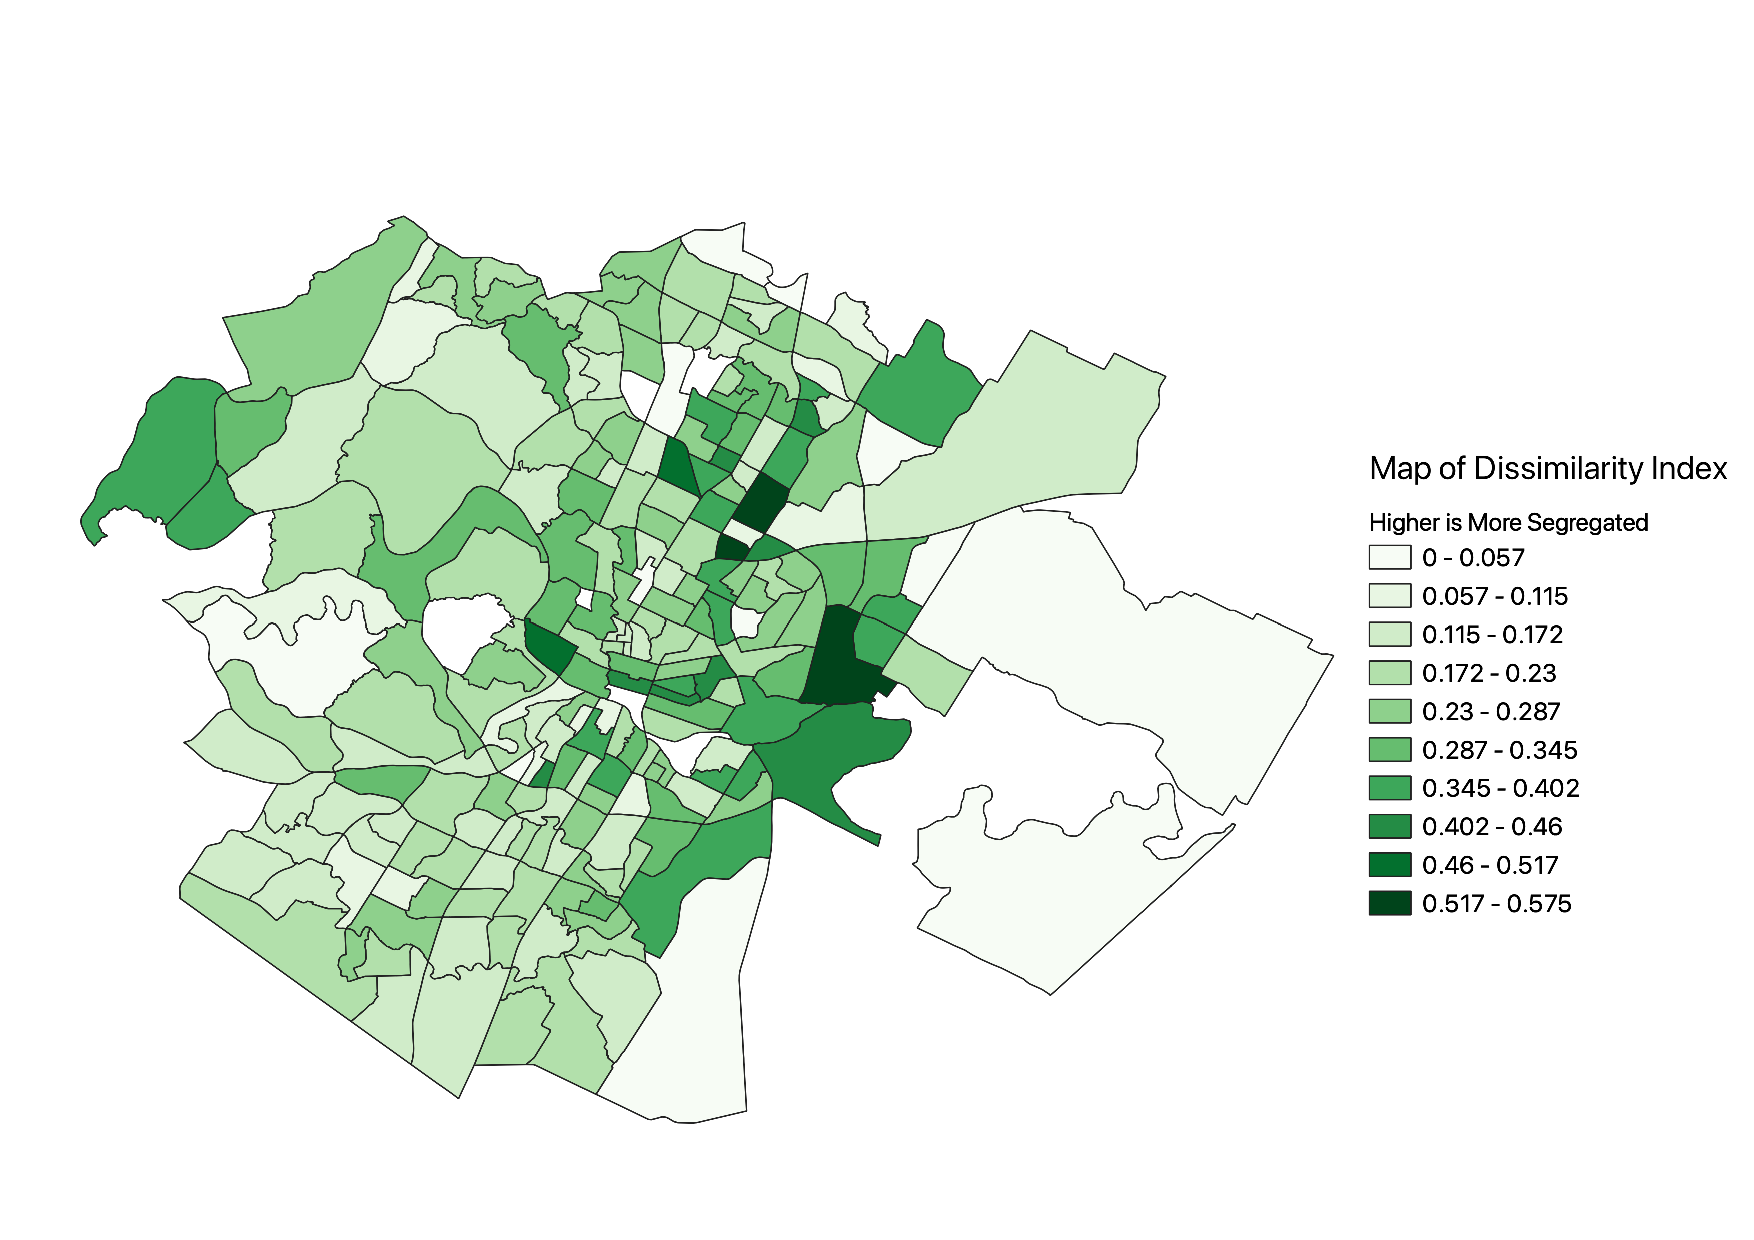
\includegraphics[width=\textwidth]{D_map_monochrome.pdf}
    \caption{Map of Austin Census Tracts by Dissimilarity Index}
    \label{fig:D_map_tracts}
\end{figure}

\begin{figure}[H]
    \centering
    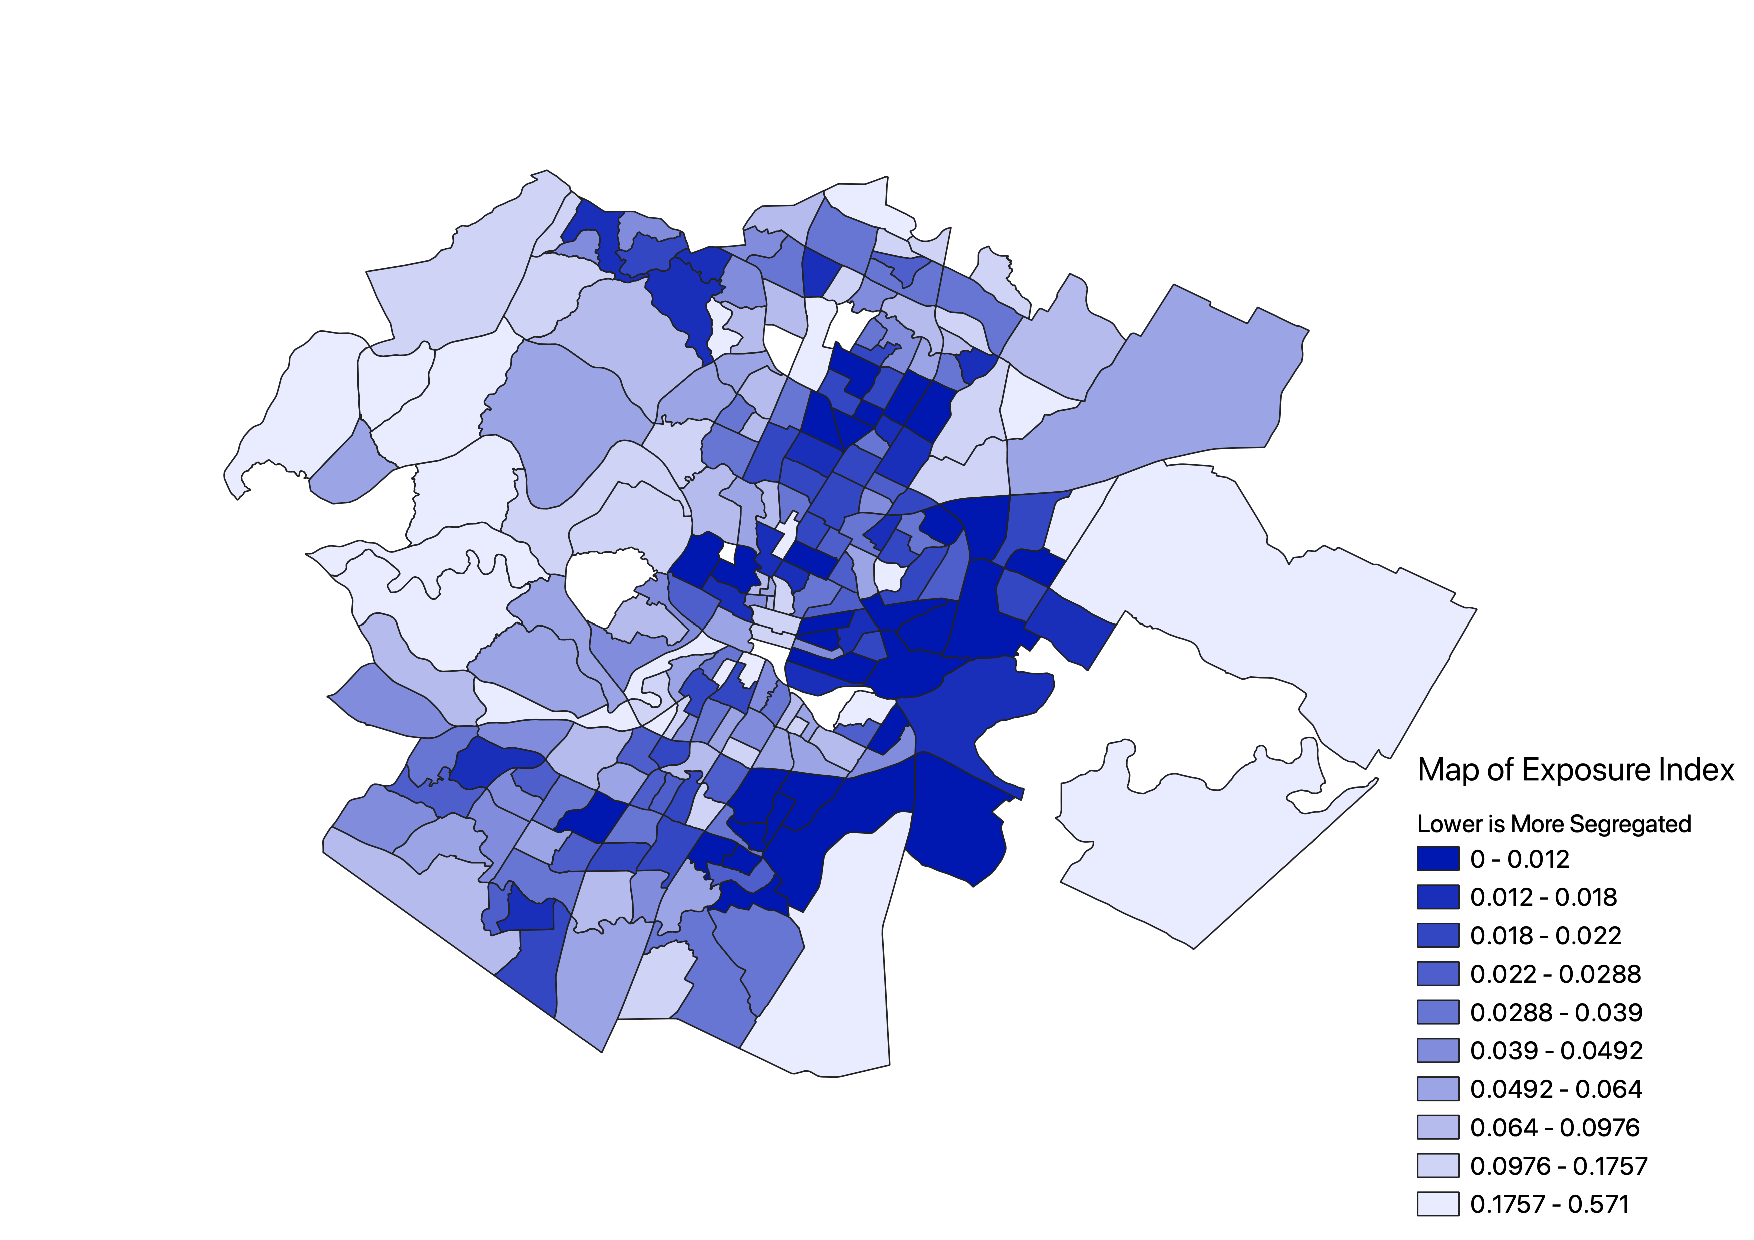
\includegraphics[width=\textwidth]{E_map_monochrome.pdf}
    \caption{Map of Austin Census Tracts by Exposure Index}
    \label{fig:E_map_tracts}
\end{figure}

I also present three measures of segregation calculated at the census block level in Austin. These maps show broad agreement, just as the measures calculated for census tracts do. This is reassuring, because throughout this paper, I use the White share as a proxy for segregation, though segregation is more nebulous and subtle than any simple demographic measure can capture fully. To quantify the relationship between the three measures, I present in Table B1 the Pearson and Spearman correlations between H, HHI, and the White Share.

\begin{table}[!htbp] 
    \centering 
  \caption{Pearson and Spearman Correlation Between Census Block Segregation Measures} 
  \label{tab:blocks_pearson} 
\begin{tabular}{@{\extracolsep{5pt}}lp{1in}p{1in}p{1in}p{0.1mm}} 
\\[-1.8ex]
\hline 
\hline 
&  \centering H & \centering HHI & \centering White Share &\\
\hline
H & \centering (1,1)&\centering ---&\centering ---&\\
HHI&\centering (-0.85, -0.85) &\centering (1,1)&\centering ---&\\
White Share &\centering (0.49, 0.61)&\centering (-0.54, -0.62)&\centering (1,1)&\\
\hline 
\hline \\[-1.8ex]
\multicolumn{4}{l}{\textit{Note:} Correlations are presented as ($r, \rho$)}
\end{tabular} 
\end{table}

\begin{figure}[H]
    \centering
    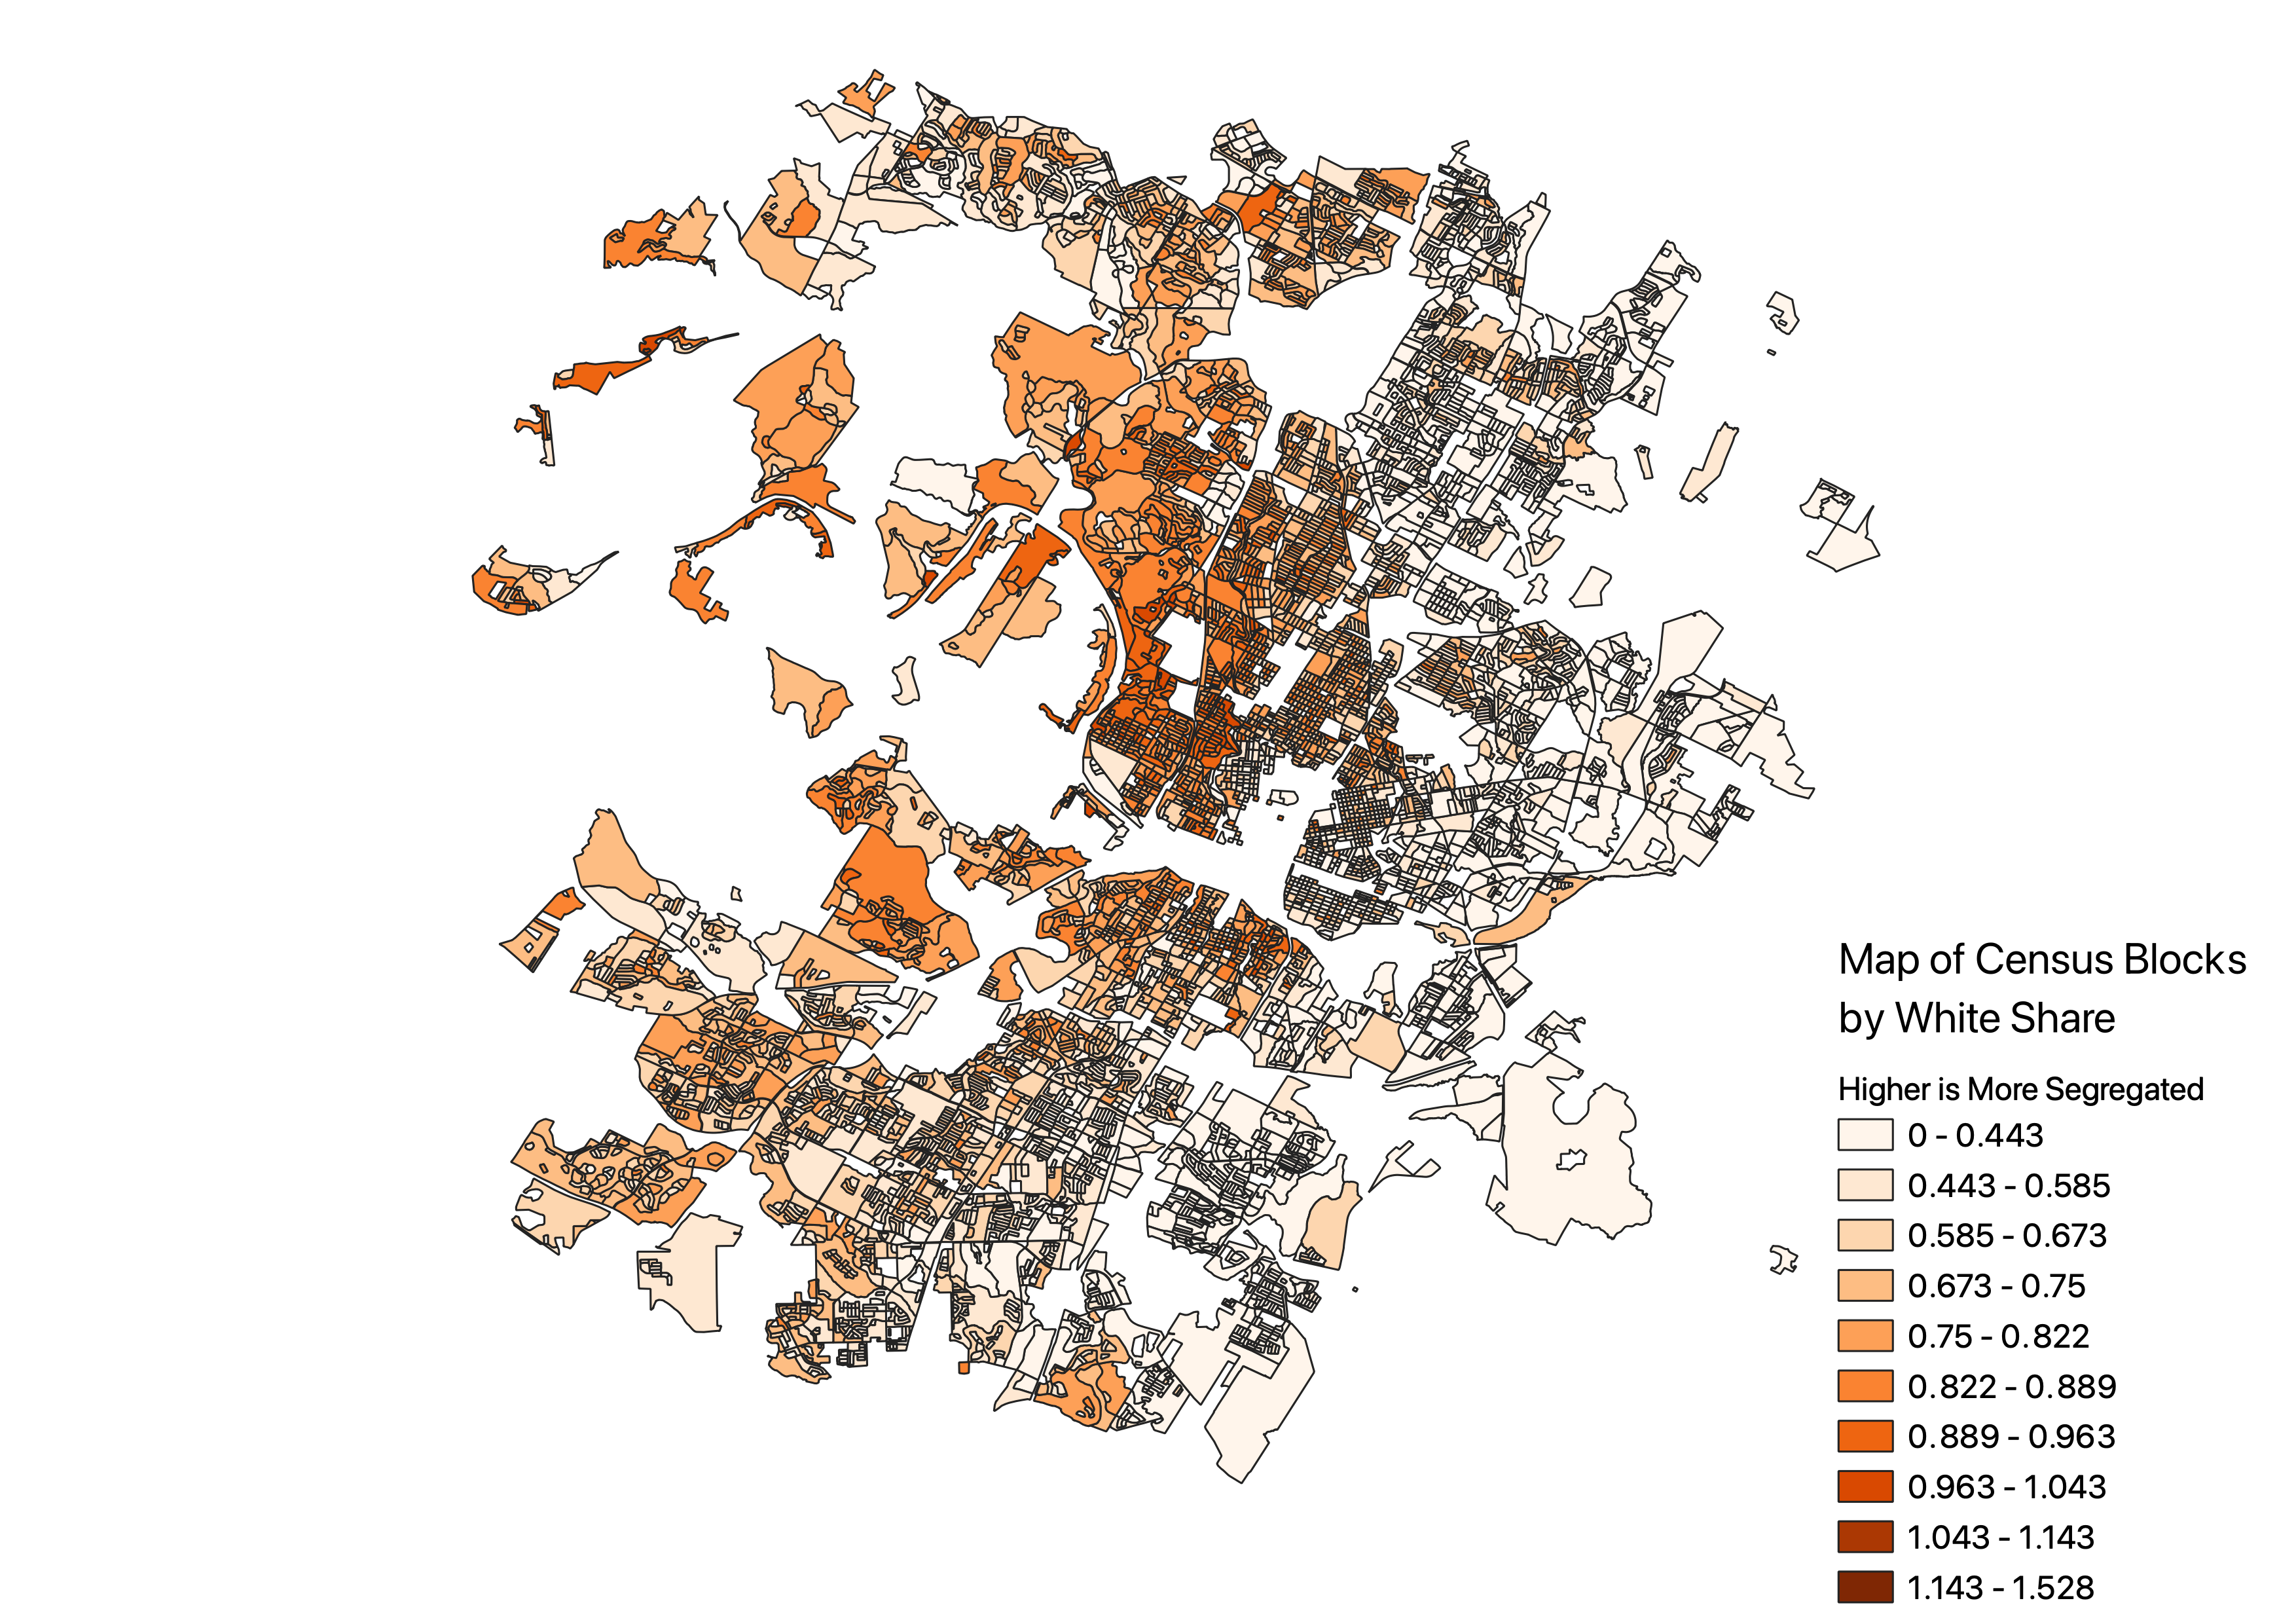
\includegraphics[width=\textwidth]{white-share_map_monochrome.png}
    \caption{Map of Austin Census Blocks by White Share}
    \label{fig:white-share_map_blocks}
\end{figure}

\begin{figure}[H]
    \centering
    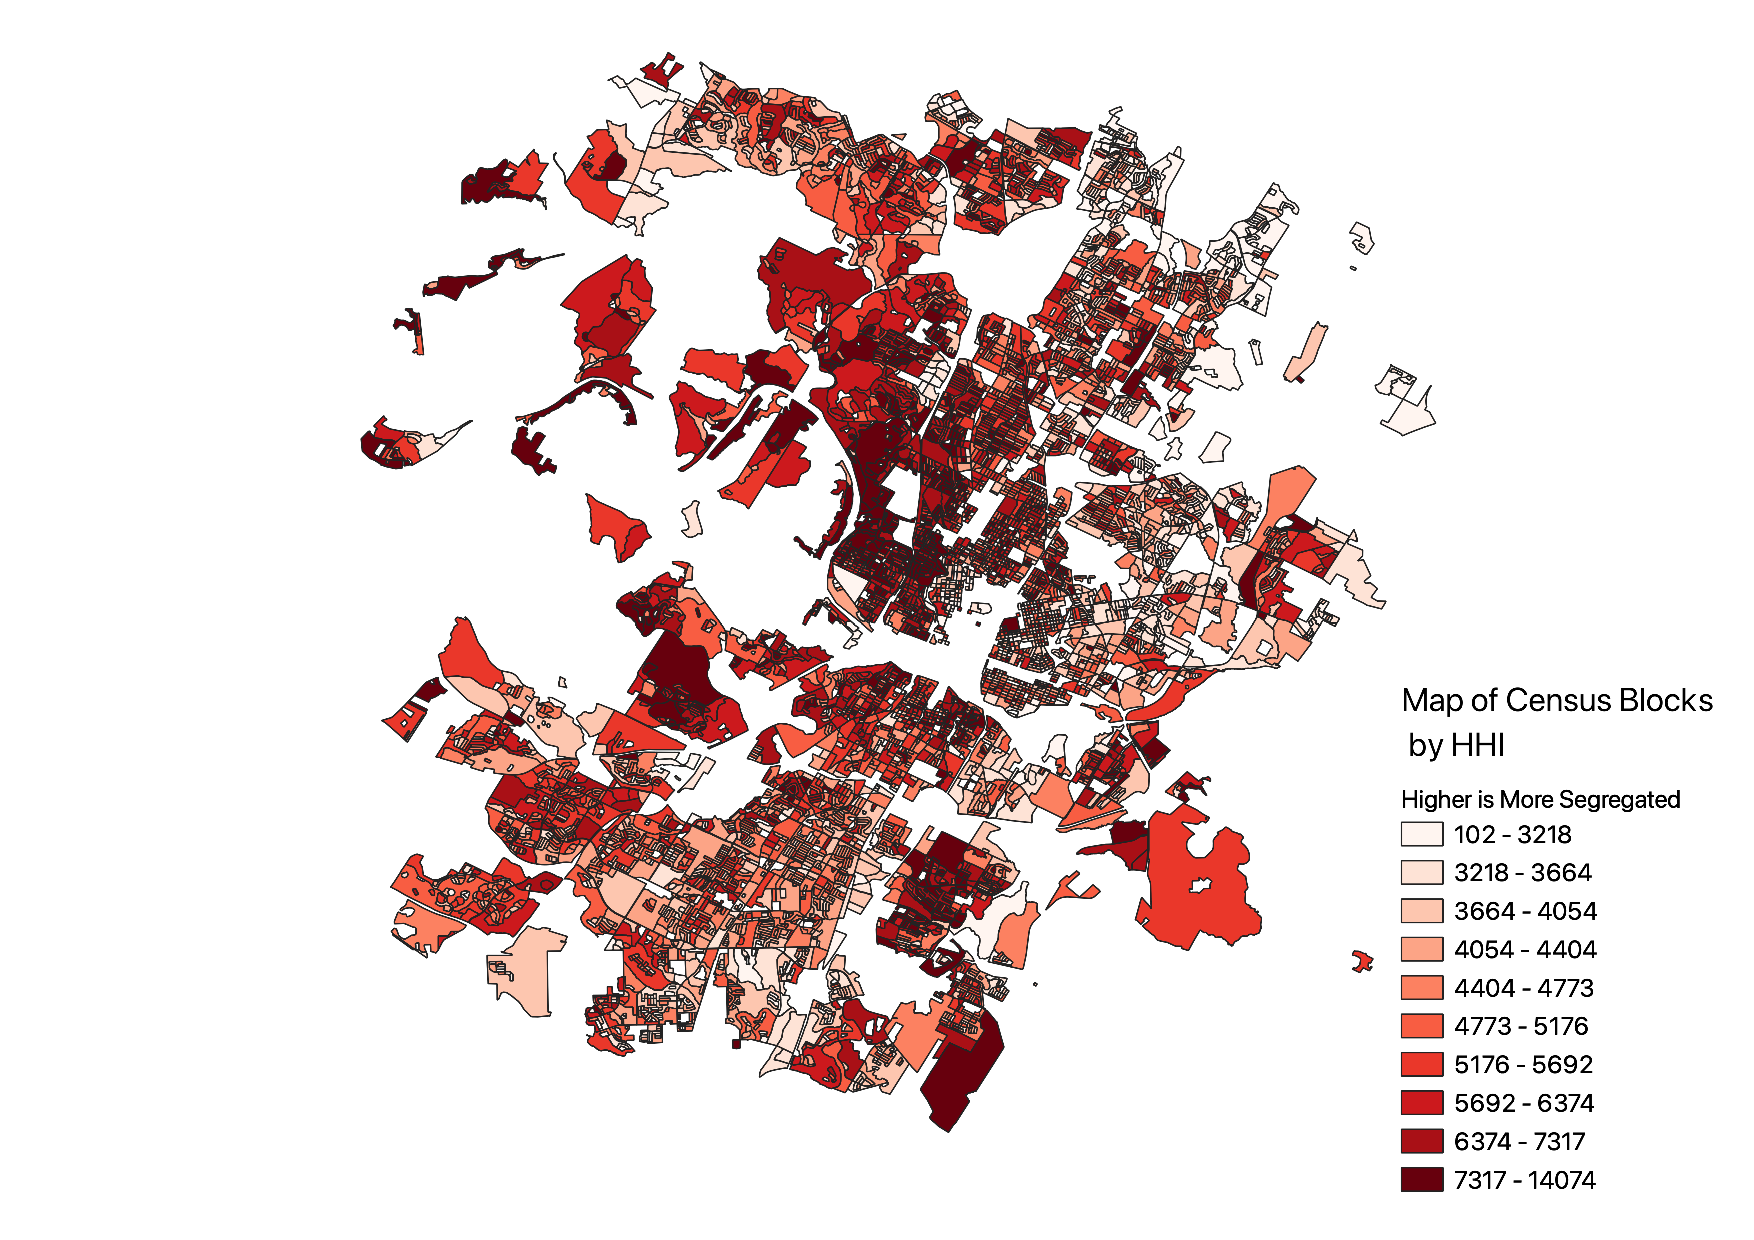
\includegraphics[width=\textwidth]{HHI_map_monochrome.pdf}
    \caption{Map of Austin Census Blocks by Herfindahl-Hirschman Index}
    \label{fig:HHI_map_blocks}
\end{figure}

\begin{figure}[H]
    \centering
    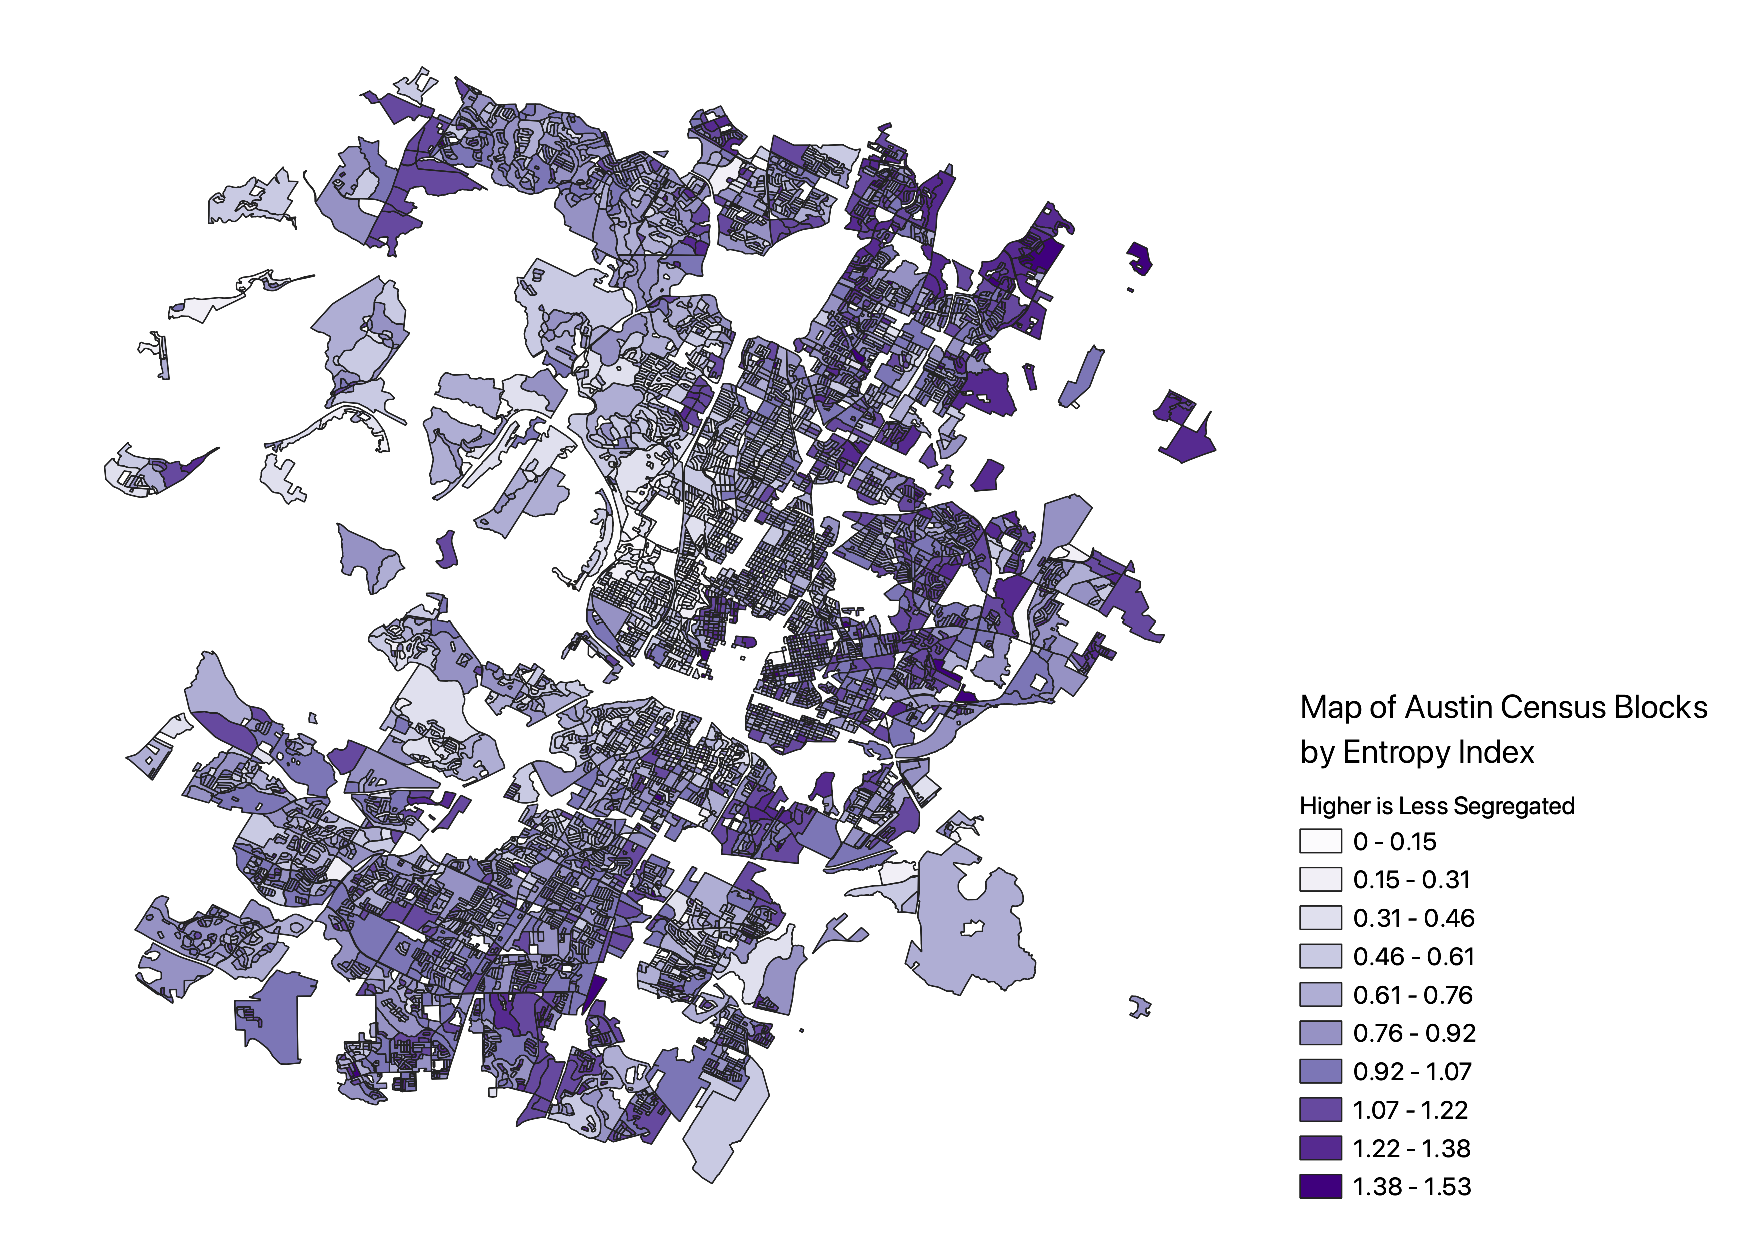
\includegraphics[width=\textwidth]{H-map_monochrome_legendFIXED.pdf}
    \caption{Map of Austin Census Blocks by Entropy Index}
    \label{fig:H_map_blocks}
\end{figure}


\pagebreak
\section*{Appendix C} 
\addcontentsline{toc}{section}{Appendix C}
\setcounter{table}{0}
\renewcommand{\thetable}{C\arabic{table}}
\setcounter{figure}{0}
\renewcommand{\thefigure}{C\arabic{figure}}

In this Appendix, I describe and illustrate the process by which I select census blocks for inclusion in the boundary dataset. In Figure \ref{fig:Austin_Zoning_Map}, I show a map of Austin Census Blocks colored by zoning generated with QGIS. So, I have information not just about how each census block is zoned, but also about each block's geography. Moreover, I have information about to which blocks a given census block is adjacent, and how those adjacent blocks. So, the spatial dataset depicted in Figure \ref{fig:Austin_Zoning_Map} contains all the information needed to restrict my sample to those blocks adjacent to zoning boundaries. In the figures below, I focus on specific parts of the map to show examples of which blocks would or would not be included.

\begin{figure}[h]
    \centering
    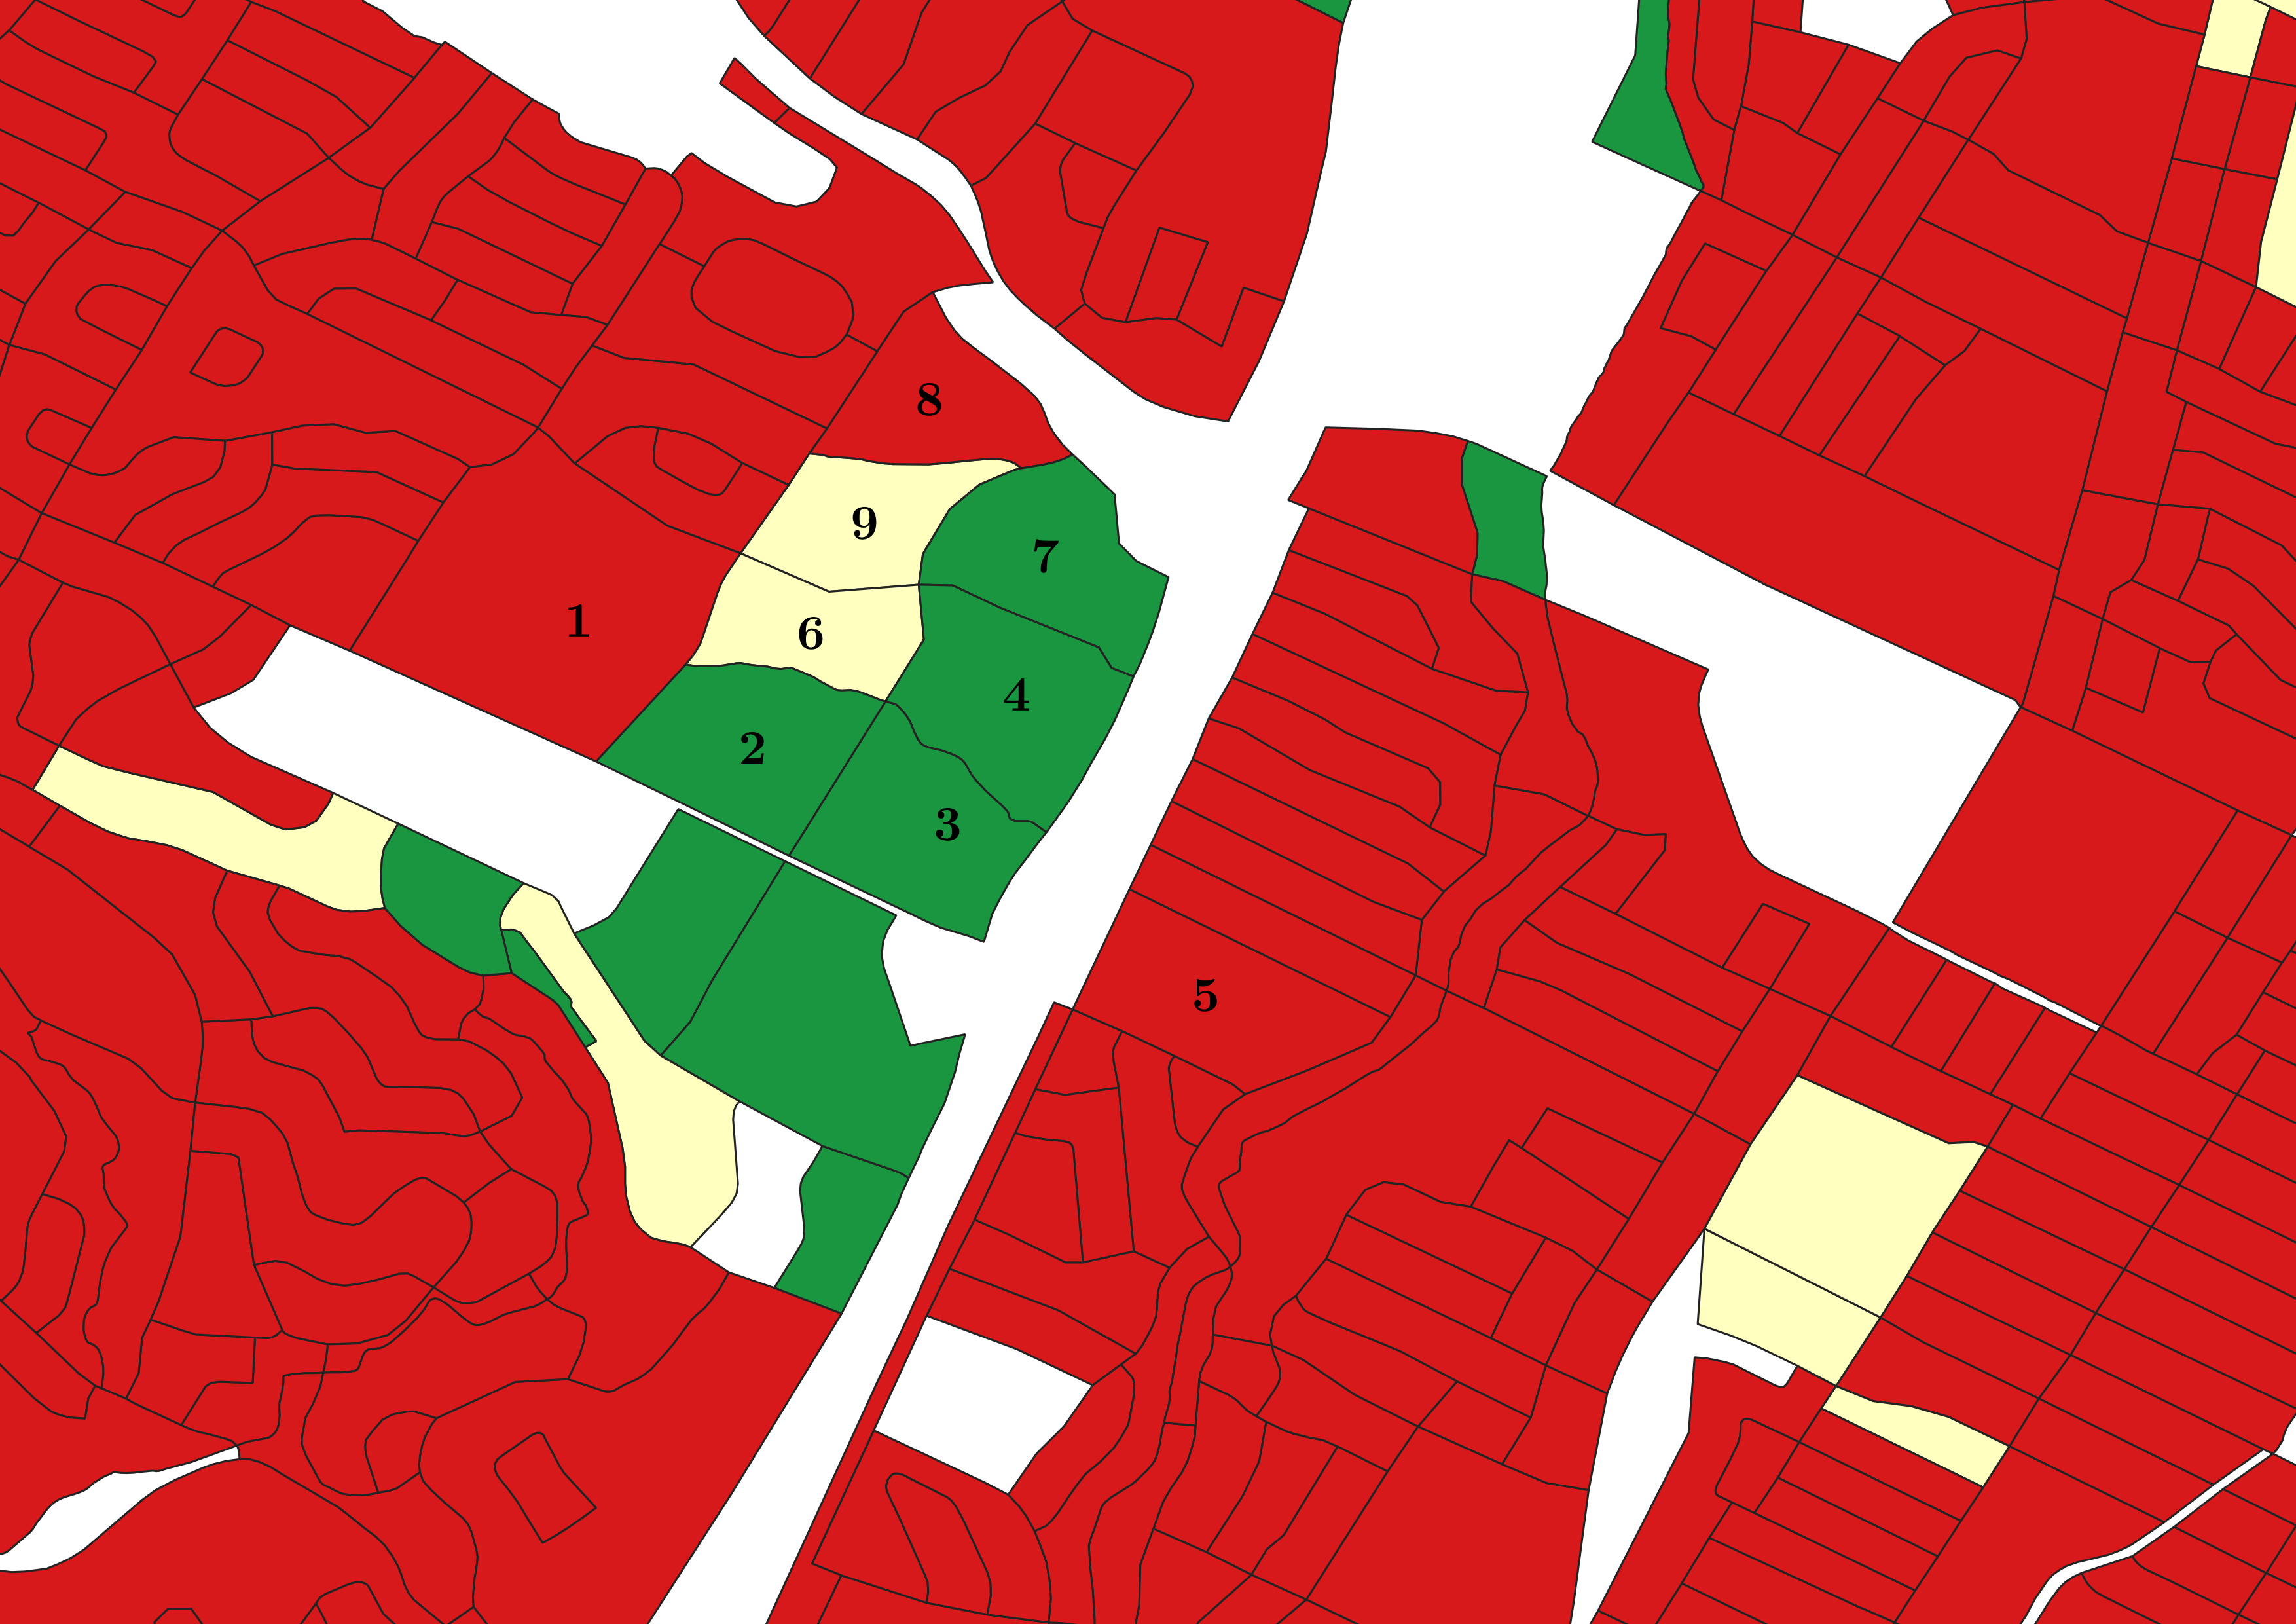
\includegraphics[width=0.8\textwidth]{selection_examplePNG.png}
    \caption{Example of Selection Process for Boundary Subset}
    \label{fig:Selection_Example1}
\end{figure}

In Figure \ref{fig:Selection_Example1}, I show a small section of the map, which is instructive in understanding how I construct my sample. I also, for convenience, add labels to several blocks, although note that the labels do not have any intrinsic meaning and are not derived from any geographic identifiers. From this section of the map, I include in the boundary dataset blocks 1 and 2. Other blocks are excluded. Although blocks 3 and 5 are adjacent, they are separated by some distance, suggesting that there is an area of non-residential land between them. This makes the exogeneity assumption less plausible and makes more difficult a causal interpretation. Accordingly, I exclude blocks 3 and 5. Blocks 6 and 9 are each zoned for some diversity of housing stock (shown by their beige color) and so they are excluded because their borders with 4 and 7 does not represent a dramatic change in zoning. Blocks 7 and 8 are excluded because their border is short relative to the size of the two blocks.

The decisions about which blocks to include in the boundary dataset are, ultimately, dependent on my judgment. I am aware that biases or errors arising from this process may affect the outcome of this research. However, two facts mitigate this risk. The first is that I explain my criteria for inclusion, and then provide a list of which blocks are included in the causal sample. The second is that---because of the nature of the QGIS software---when I pick tracts for inclusion in the causal sample, I cannot see the racial composition of those blocks. This means I cannot influence the outcome by selecting only those blocks whose combination of zoning and racial makeup is favorable to obtaining significant results. Below, in Figure \ref{fig:Causal_Map}, I display the tracts which I include in the boundary subset (\textit{cf.} Figure \ref{fig:Austin_Zoning_Map}), and their zoning.

\begin{figure}[h]
    \centering
    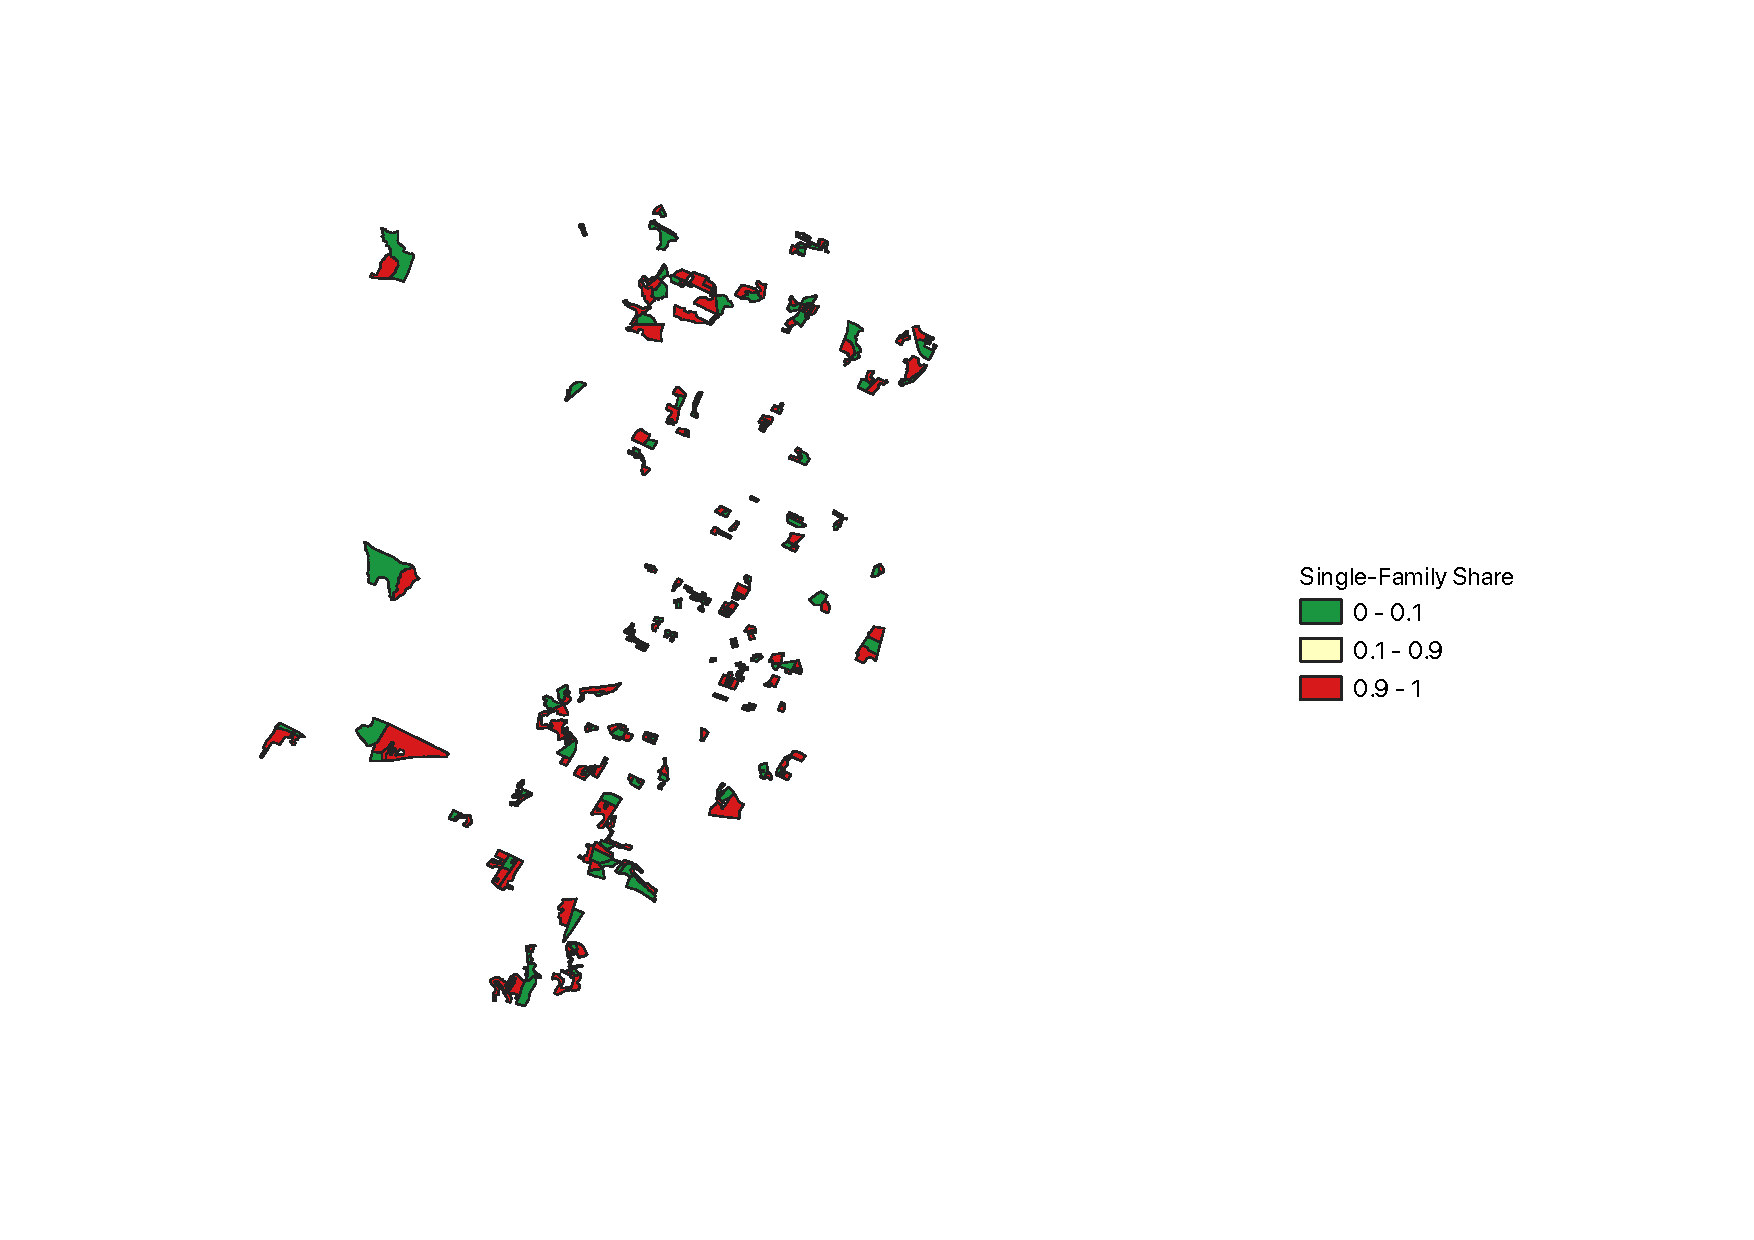
\includegraphics[width=\textwidth]{fig_2_causal_redone.pdf}
    \caption{Map of Boundary Subset of Census Blocks}
    \label{fig:Causal_Map}
\end{figure}

\clearpage
\section*{Appendix D} 
\addcontentsline{toc}{section}{Appendix D}
\setcounter{table}{0}
\renewcommand{\thetable}{D\arabic{table}}

\setcounter{figure}{0}
\renewcommand{\thefigure}{D\arabic{figure}}

I create an indicator variable equal to $1$ when the geocoder matches an address and $0$ when the geocoder fails to produce a match. Then, I estimate a model of the probability of matching, taking the zoning categories as a predictor. The reference category is \textit{Multi-Family Highest Density}. Ideally, no zoning category would be significantly predictive of matching, yet some of the zoning indicator variables are highly statistically significant. Table D1, below, shows the results from both a logistic regression and an OLS regression where single- and multi-family categories are collapsed, and multi-family is the reference category. The coefficient on Single-Family is 0.065, indicating that single-family addresses are 6.5 percentage points more likely to match. Next, I test whether disaggregating the zoning categories (i.e., using individual zoning categories as predictors) alleviates this problem. In Table D2, I show that there are still significant differences in the probability of matching for addresses zoned for single- versus multi-family housing.

\begin{table}[!htbp] \centering 
  \caption{Simple Comparison of Matched and Unmatched Addresses} 
  \label{tab:geocode_match_biv} 
\begin{tabular}{@{\extracolsep{5pt}}lcc} 
\\[-1.8ex]\hline 
\hline \\[-1.8ex] 
 & \multicolumn{2}{c}{\textit{Dependent variable:}} \\ 
\cline{2-3} 
\\[-1.8ex] & \multicolumn{2}{c}{Match} \\ 
\\[-1.8ex] & \textit{OLS} & \textit{Logistic} \\ 
\\[-1.8ex] & (1) & (2)\\ 
\hline \\[-1.8ex] 
 Single-Family & 0.065$^{***}$ & 0.755$^{***}$ \\ 
  & (0.004) & (0.035) \\ 
  & & \\ 
 Constant & 0.869$^{***}$ & 1.889$^{***}$ \\ 
  & (0.004) & (0.034) \\ 
  & & \\ 
\hline \\[-1.8ex] 
Observations & 183,378 & 183,378 \\ 
Adjusted R$^{2}$ & 0.003 &  \\ 
Log Likelihood &  & $-$45,911.920 \\ 
Akaike Inf. Crit. &  & 91,827.850 \\ 
\hline 
\hline \\[-1.8ex] 
\textit{Note:} Robust Standard Errors in Parentheses. & \multicolumn{2}{r}{$^{*}$p$<$0.1; $^{**}$p$<$0.05; $^{***}$p$<$0.01} \\ 
\end{tabular} 
\end{table} 



\begin{table}[!htbp] \centering 
  \caption{Detailed Comparison of Matched and Unmatched Addresses} 
  \label{tab:geocode_match_categorical} 
\begin{tabular}{@{\extracolsep{5pt}}lcc} 
\\[-1.8ex]\hline 
\hline \\[-1.8ex] 
 & \multicolumn{2}{c}{\textit{Dependent variable:}} \\ 
\cline{2-3} 
\\[-1.8ex] & \multicolumn{2}{c}{Match} \\ 
\\[-1.8ex] & \textit{OLS} & \textit{Logistic} \\ 
\\[-1.8ex] & (1) & (2)\\ 
\hline \\[-1.8ex] 
 Multi-Family Limited Density & $-$0.093$^{***}$ & $-$1.462$^{***}$ \\ 
  & (0.013) & (0.388) \\ 
  & & \\ 
 Multi-Family Moderate Density & $-$0.134$^{***}$ & $-$1.789$^{***}$ \\ 
  & (0.014) & (0.388) \\ 
  & & \\ 
 Multi-Family Moderate High Density & $-$0.061$^{***}$ & $-$1.124$^{***}$ \\ 
  & (0.014) & (0.394) \\ 
  & & \\ 
 Single-Family Large Lot & 0.004 & 0.151 \\ 
  & (0.012) & (0.390) \\ 
  & & \\ 
 Single-Family Residence & 0.008 & 0.305 \\ 
  & (0.012) & (0.385) \\ 
  & & \\ 
 Single-Family Small Lot & $-$0.350$^{***}$ & $-$2.920$^{***}$ \\ 
  & (0.013) & (0.385) \\ 
  & & \\ 
 Single-Family Standard Lot & $-$0.013 & $-$0.348 \\ 
  & (0.012) & (0.385) \\ 
  & & \\ 
 Constant & 0.968$^{***}$ & 3.401$^{***}$ \\ 
  & (0.012) & (0.384) \\ 
  & & \\ 
\hline \\[-1.8ex] 
Observations & 183,378 & 183,378 \\ 
Adjusted R$^{2}$ & 0.157 &  \\ 
Log Likelihood &  & $-$37,250.830 \\ 
Akaike Inf. Crit. &  & 74,517.660 \\ 
\hline 
\hline \\[-1.8ex] 
\textit{Note:} Robust Standard Errors in Parentheses.  & \multicolumn{2}{r}{$^{*}$p$<$0.1; $^{**}$p$<$0.05; $^{***}$p$<$0.01} \\ 
\end{tabular} 
\end{table} 

\clearpage

\section*{Appendix E} 
\addcontentsline{toc}{section}{Appendix E}

\setcounter{table}{0}
\renewcommand{\thetable}{E\arabic{table}}

\setcounter{figure}{0}
\renewcommand{\thefigure}{E\arabic{figure}}

\begin{table}[!htbp] \centering 
  \caption{Bivariate Regression on Sophisticated Segregation Measures, Boundary Subset} 
  \label{tab:naive_biv_sophisticated_causal} 
\begin{tabular}{@{\extracolsep{5pt}}lcc} 
\\[-1.8ex]\hline 
\hline \\[-1.8ex] 
 & \multicolumn{2}{c}{\textit{Dependent variable:}} \\ 
\cline{2-3} 
\\[-1.8ex] & Entropy Index & HHI \\ 
\\[-1.8ex] & (1) & (2)\\ 
\hline \\[-1.8ex] 
 Single Family Share & $-$0.102$^{***}$ & 522.757$^{***}$ \\ 
  & (0.027) & (159.031) \\ 
  & & \\ 
\hline \\[-1.8ex] 
Observations & 332 & 332 \\ 
Adjusted R$^{2}$ & 0.037 & 0.028 \\  
\hline 
\hline \\[-1.8ex] 
\multicolumn{3}{l}{\textit{Note:} Robust Standard Errors in Parentheses. $^{*}$p$<$0.1; $^{**}$p$<$0.05; $^{***}$p$<$0.01} \\ 
\end{tabular} 
\end{table} 


\begin{table}[!htbp] \centering 
  \caption{Logistic Estimates with Controls, Boundary Subset} 
  \label{tab:logit_controls_causal} 
\begin{tabular}{@{\extracolsep{5pt}}lccccc} 
\\[-1.8ex]\hline 
\hline \\[-1.8ex] 
 & \multicolumn{5}{c}{\textit{Dependent variable:}} \\ 
\cline{2-6} 
\\[-1.8ex] & \multicolumn{5}{c}{White Share} \\ 
\\[-1.8ex] & (1) & (2) & (3) & (4) & (5)\\ 
\hline \\[-1.8ex] 
 Single Family Share & 0.295$^{***}$ & 0.285$^{***}$ & 0.386$^{***}$ & 0.392$^{***}$ & 0.267$^{**}$ \\ 
  & (0.106) & (0.111) & (0.112) & (0.119) & (0.111) \\ 
  & & & & & \\ 
\hline \\[-1.8ex] 
Observations & 332 & 332 & 332 & 332 & 332\\ 
Log Likelihood & $-$221.291 & $-$226.566 & $-$166.434 & $-$166.433 & $-$221.018 \\ 
Akaike Inf. Crit. & 448.583 & 459.131 & 530.868 & 532.865 & 450.035 \\ 
\hline
Income & Y & N & N & N & Y\\
Population & N & Y & N & Y & Y\\
Tract FE & N & N & Y & Y & N\\
\hline 
\hline \\[-1.8ex] 
\multicolumn{6}{l}{\textit{Note:} Robust Standard Errors in Parentheses. $^{*}$p$<$0.1; $^{**}$p$<$0.05; $^{***}$p$<$0.01} \\
\end{tabular} 
\end{table} 
\pagebreak

\begin{table}[!htbp] \centering 

  \caption{Regressions on the Entropy Index, Boundary Subset} 
  \label{tab:Entropy_Causal} 
\begin{tabular}{@{\extracolsep{5pt}}lccccc} 
\\[-1.8ex]\hline 
\hline \\[-1.8ex] 
 & \multicolumn{5}{c}{\textit{Dependent variable:}} \\ 
\cline{2-6} 
\\[-1.8ex] & \multicolumn{5}{c}{Entropy Index} \\ 
\\[-1.8ex] & (1) & (2) & (3) & (4) & (5)\\ 
\hline \\[-1.8ex] 
 Single Family Share & $-$0.093$^{***}$ & $-$0.066$^{**}$ & $-$0.094$^{***}$ & $-$0.076$^{***}$ & $-$0.061$^{**}$ \\ 
  & (0.027) & (0.027) & (0.026) & (0.027) & (0.027) \\ 
  & & & & & \\ 
\hline \\[-1.8ex] 
Observations & 332 & 332 & 332 & 332 & 332 \\ 
Adjusted R$^{2}$ & 0.092 & 0.101 & 0.297 & 0.312 & 0.144 \\ 
\hline
Income Control & Y & N & N & N & Y\\
Population Control & N & Y & N & Y & Y\\
Tract FE & N & N & Y & Y & N\\
\hline 
\hline \\[-1.8ex] 
\multicolumn{6}{l}{\textit{Note:} Robust Standard Errors in Parentheses. $^{*}$p$<$0.1; $^{**}$p$<$0.05; $^{***}$p$<$0.01} \\
\end{tabular} 
\end{table} 


\begin{table}[!htbp] \centering 
  \caption{Regressions on the Herfindahl-Hirschman Index, Boundary Subset} 
  \label{tab:HHI_Causal} 
\begin{tabular}{@{\extracolsep{5pt}}lccccc} 
\\[-1.8ex]\hline 
\hline \\[-1.8ex] 
 & \multicolumn{5}{c}{\textit{Dependent variable:}} \\ 
\cline{2-6} 
\\[-1.8ex] & \multicolumn{5}{c}{Herfindahl-Hirschman Index} \\ 
\\[-1.8ex] & (1) & (2) & (3) & (4) & (5)\\ 
\hline \\[-1.8ex] 
 Single Family Share & 478.664$^{***}$ & 408.978$^{**}$ & 526.791$^{***}$ & 498.155$^{***}$ & 384.016$^{**}$ \\ 
  & (157.522) & (162.471) & (161.051) & (166.120) & (161.007) \\ 
  & & & & & \\ 
\hline \\[-1.8ex] 
Observations & 332 & 332 & 332 & 332 & 332 \\ 
Adjusted R$^{2}$ & 0.061 & 0.043 & 0.210 & 0.208 & 0.072 \\ 
\hline
Income Control & Y & N & N & N & Y\\
Population Control & N & Y & N & Y & Y\\
Tract FE & N & N & Y & Y & N\\
\hline 
\hline \\[-1.8ex] 
\multicolumn{6}{l}{\textit{Note:} Robust Standard Errors in Parentheses. $^{*}$p$<$0.1; $^{**}$p$<$0.05; $^{***}$p$<$0.01} \\
\end{tabular} 
\end{table} 


\end{document}